
  % ------------------------------------------------------------------------
  % abnTeX2: Modelo de Trabalho Academico (tese de doutorado, dissertacao de
  % mestrado e trabalhos monograficos em geral) em conformidade com
  % ABNT NBR 14724:2011: Informacao e documentacao - Trabalhos academicos -
  % Apresentacao
  % ------------------------------------------------------------------------
  % ------------------------------------------------------------------------

  \documentclass[
    % -- opções da classe memoir --
    12pt,       % tamanho da fonte
    openright,      % capítulos começam em pág ímpar (insere página vazia caso preciso)
    twoside,      % para impressão em verso e anverso. Oposto a oneside
    a4paper,      % tamanho do papel.
    % -- opções da classe abntex2 --
    %chapter=TITLE,   % títulos de capítulos convertidos em letras maiúsculas
    %section=TITLE,   % títulos de seções convertidos em letras maiúsculas
    %subsection=TITLE,  % títulos de subseções convertidos em letras maiúsculas
    %subsubsection=TITLE,% títulos de subsubseções convertidos em letras maiúsculas
    % -- opções do pacote babel --
    english,      % idioma adicional para hifenização
    french,       % idioma adicional para hifenização
    spanish,      % idioma adicional para hifenização
    brazil,       % o último idioma é o principal do documento
    ]{abntex2}


  % ---
  % PACOTES
  % ---

  % ---
  % Pacotes fundamentais
  % ---
  \usepackage{cmap}       % Mapear caracteres especiais no PDF
  \usepackage{lmodern}      % Usa a fonte Latin Modern
  \usepackage[T1]{fontenc}    % Selecao de codigos de fonte.
  \usepackage[utf8]{inputenc}   % Codificacao do documento (conversão automática dos acentos)
  \usepackage{lastpage}     % Usado pela Ficha catalográfica
  \usepackage{indentfirst}    % Indenta o primeiro parágrafo de cada seção.
  \usepackage{color}        % Controle das cores
  \usepackage{graphicx}     % Inclusão de gráficos
  \usepackage{listings}     % Inclusão de código
  \usepackage[final]{pdfpages}
  \usepackage{algorithm}
  \usepackage{algorithmic}
  \usepackage{color}
  \usepackage[section]{placeins}
  \usepackage{csquotes}
  \usepackage{longtable}
  \usepackage[table]{xcolor}
  \usepackage{multirow}
  \usepackage{pdfpages}
  
  \definecolor{shadecolor}{rgb}{0.8,0.8,0.8}

  % ---
  % Pacotes de citações
  % ---
  \usepackage[brazilian,hyperpageref]{backref}   % Paginas com as citações na bibl
  \usepackage[alf]{abntex2cite} % Citações padrão ABNT

  % ---
  % CONFIGURAÇÕES DE PACOTES
  % ---

  % ---
  % Configurações do pacote backref
  % Usado sem a opção hyperpageref de backref
  \renewcommand{\backrefpagesname}{Citado na(s) página(s):~}
  % Texto padrão antes do número das páginas
  \renewcommand{\backref}{}
  % Define os textos da citação
  \renewcommand*{\backrefalt}[4]{
    \ifcase #1 %
      Nenhuma citação no texto.%
    \or
      Citado na página #2.%
    \else
      Citado #1 vezes nas páginas #2.%
    \fi}%
    
\renewcommand{\lstlistingname}{Código}
  % ---

  % ---
  % Informações de dados para CAPA e FOLHA DE ROSTO
  % ---
  \titulo{Um estudo de caso de gestão de riscos aplicada a métodos ágeis}
  \autor{Fernanda Narloch Rizzo Hahn}
  \local{Florianópolis}
  \data{2022}
  \orientador{Jean Carlo Rossa Hauck}
  \coorientador{}
  \instituicao{%
    Universidade Federal de Santa Catarina
    \par
    Centro Tecnológico - CTC
    \par
    Departamento de Informática e Estatística
    \par
    Ciências da Computação}
  \tipotrabalho{Dissertação (Bacharelado)}

  \preambulo{Trabalho de Conclusão de Curso submetido ao Curso de
  Ciências da Computação para a obtenção do Grau de Bacharel em
  Ciências da Computação.}
  % ---

  % ---
  % Configurações de aparência do PDF final
    \def\changemargin#1#2{\list{}{\rightmargin#2\leftmargin#1}\item[]}
    \let\endchangemargin=\endlist 

  % alterando o aspecto da cor azul
  \definecolor{blue}{RGB}{41,5,195}

  % informações do PDF
  \makeatletter
  \hypersetup{
        %pagebackref=true,
      pdftitle={\@title},
      pdfauthor={\@author},
        pdfsubject={\imprimirpreambulo},
        pdfcreator={LaTeX with abnTeX2},
      pdfkeywords={abnt}{latex}{abntex}{abntex2}{trabalho acadêmico},
      colorlinks=true,          % false: boxed links; true: colored links
        linkcolor=black,           % color of internal links
        citecolor=black,           % color of links to bibliography
        filecolor=magenta,          % color of file links
      urlcolor=blue,
      bookmarksdepth=4
  }
  \makeatother
  % ---
  % ---
  % Espaçamentos entre linhas e parágrafos
  % ---

  % O tamanho do parágrafo é dado por:
  \setlength{\parindent}{1.3cm}

  % Controle do espaçamento entre um parágrafo e outro:
  \setlength{\parskip}{0.2cm}  % tente também \onelineskip

  % ---
  % compila o indice
  % ---
  \makeindex
  % ---
    % \hypersetup{draft}
  % ----
  % Início do documento
  % ----
  \begin{document}
  % Retira espaço extra obsoleto entre as frases.
  \frenchspacing

  % ----------------------------------------------------------
  % ELEMENTOS PRÉ-TEXTUAIS
  % ----------------------------------------------------------
  % \pretextual

  % ---
  % Capa
  % ---
  \imprimircapa
  % ---

  % ---
  % Folha de rosto
  % (o * indica que haverá a ficha bibliográfica)
  % ---
  \imprimirfolhaderosto*
  % ---
  
  % ---
  % Inserir folha de aprovação
  % ---

  % Isto é um exemplo de Folha de aprovação, elemento obrigatório da NBR
  % 14724/2011 (seção 4.2.1.3). Você pode utilizar este modelo até a aprovação
  % do trabalho. Após isso, substitua todo o conteúdo deste arquivo por uma
  % imagem da página assinada pela banca com o comando abaixo:
  %
  % \includepdf{folhadeaprovacao_final.pdf}
  %
  \begin{folhadeaprovacao}

    \begin{center}
      {\ABNTEXchapterfont\large\imprimirautor}

      \vspace*{\fill}
      {\ABNTEXchapterfont\large\bfseries\imprimirtitulo}
      \vspace*{\fill}


     Este Trabalho de Conclusão de Curso foi julgado aprovado para a
     obtenção do Título de Bacharel em Ciências da Computação, e
     aprovado em sua forma final pelo Curso de Ciências da Computação
     da Universidade Federal de Santa Catarina.
     \end{center}

     \assinatura{Dr. Prof. \imprimirorientador \\ Orientador}
     \assinatura{Dr. Prof. Raul Sidnei Wazlawick  \\ Avaliador}
     \assinatura{M.e. Thaísa Cardoso Lacerda  \\ Avaliador}
     %\assinatura{\textbf{Professor} \\ Convidado 3}
     %\assinatura{\textbf{Professor} \\ Convidado 4}

     \begin{center}
      \vspace*{0.5cm}
      {\large\imprimirlocal}
      \par
      {\large\imprimirdata}
      \vspace*{1cm}
    \end{center}

  \end{folhadeaprovacao}
  % ---

  % ---
  % Agradecimentos
  % ---
  \begin{agradecimentos}
  \end{agradecimentos}
  % ---

  % ---
  % Epígrafe
  % ---
  \begin{epigrafe}
      \vspace*{\fill}
    \begin{flushright}
      \textit{“As long as you are learning, you are not failing.” – Bob Ross}
    \end{flushright}
  \end{epigrafe}
  % ---

  % ---
  % RESUMOS
  % ---

  % resumo em português
  \begin{resumo}
    A popularização dos métodos ágeis no desenvolvimento de \textit{\textit{software}} trouxe maior velocidade e flexibilidade aos projetos que anteriormente eram desenvolvidos com base em modelos prescritivos. Contudo, os métodos ágeis não são capazes de prevenir por si características típicas de projetos de \textit{software} como a imprevisibilidade e instabilidade. Pois, esses modelos de gerência de projeto não contam com técnicas formais de gestão de riscos para lidar com as incertezas existentes durante o desenvolvimento. Essa lacuna pode provocar o fracasso de um ou mais objetivos do projeto ao preterir a identificação de riscos potencias e consequentemente não dispor de um plano de contingência. Dessa forma, foi criado o “Guia para gestão ágil de riscos em projetos de \textit{software}” no contexto do Grupo de Qualidade de \textit{Software} (GQS/INE/CTC/UFSC) com o intuito de apresentar diretrizes que visam auxiliar a prática da gestão explícita de riscos no ambiente de desenvolvimento ágil de \textit{software}. Assim, o presente trabalho se trata de um estudo de caso que pretende aplicar e avaliar técnicas de gestão de riscos do Guia em equipes ágeis do Laboratório Bridge da Universidade Federal de Santa Catarina. Para isso, inicialmente serão revisados conceitos fundamentais referentes ao tema e também será realizada a análise do estado da arte na área. Com base nos conhecimentos adquiridos e no “Guia para gestão ágil de riscos em projetos de \textit{software}” será desenvolvido um diagnóstico inicial do contexto do Laboratório Bridge e, a partir dele, serão propostas as técnicas a serem aplicadas durante o estudo de caso. Após a implantação das técnicas, será realizada a avaliação dos resultados obtidos.
   \vspace{\onelineskip}

   \noindent
   \textbf{Palavras-chaves}: Gestão de Riscos, Gestão de Projetos, Métodos Ágeis, Desenvolvimento de \textit{Software}
  \end{resumo}

  % resumo em inglês
  \begin{resumo}[Abstract]

The popularization of agile methods in the development of software brought greater speed and flexibility to projects that were previously developed based on prescriptive models. However, agile methods are not able to prevent by themselves typical features of software projects such as unpredictability and instability. As these project management models do not rely on formal risk management techniques to deal with the uncertainties that exist during development. This gap can cause the failure of one or more project objectives by neglecting the identification of potential risks and consequently not having a contingency plan. Thus, the 'Guide for agile risk management in software projects' was created in the context of the 'Grupo de Qualidade de Software' (Software Quality Group, GQS/INE/CTC/UFSC) in order to present guidelines that aim to help the practice of explicit risk management in the agile development environment of software. Thus, the present work is a case study that intends to apply and evaluate risk management techniques from the Guide in agile teams at the Bridge Laboratory of the Federal University of Santa Catarina (UFSC). For this, fundamental concepts regarding the theme will be initially reviewed and an analysis of the state of the art in the area will also be carried out. Based on the acquired knowledge and on the 'Guide for agile risk management in software projects' an initial diagnosis of the Bridge Laboratory context will be developed and, in this regard, the techniques to be applied during the case study will be selected. After the implementation of the techniques, the results obtained will be evaluated.

\vspace{\onelineskip}

   \noindent
   \textbf{Palavras-chaves}: Risk Management, Project Management, Agile Methods, Software Development
  \end{resumo}
  % ---

  % ---
  % inserir lista de ilustrações
  % ---
  \pdfbookmark[0]{\listfigurename}{lof}
  \listoffigures*
  \cleardoublepage
  % ---

  % ---
  % inserir lista de tabelas
  % ---
  \pdfbookmark[0]{\listtablename}{lot}
  \listoftables*
  \cleardoublepage
  % ---

  % ---
  % inserir lista de abreviaturas e siglas
  % ---
  \begin{siglas}
    \item[PMBOK] Project Management Body of Knowledge
    \item[PMI]  Project Management Institute
    \item[UFSC] Universidade Federal de Santa Catarina
    \item[MSL] Mapeamento Sistemático da Literatura
    \item[WIP] Work in Progress
    \item[CEO] Chief Executive Officer
    \item[CXO] Chief Experience Officer
    \item[COO] Chief Operating Officer
    \item[CFO] Chief Financial Officer
    \item[SM] Scrum Master
    \item[PO] Product Owner
    \item[PEC] Prontuário Eletrônico do Cidadão
    \item[GQM] Goal/Question/Metric

 \end{siglas}
  % ---

  % ---
  % inserir o sumario
  % ---
  \pdfbookmark[0]{\contentsname}{toc}
  \tableofcontents*
  \cleardoublepage
  % ---



  % ----------------------------------------------------------
  % ELEMENTOS TEXTUAIS
  % ----------------------------------------------------------
  \textual


  % ----------------------------------------------------------
  % PARTE - preparação da pesquisa
  % ----------------------------------------------------------
\chapter{Introdução e objetivos}
\label{sec:Introducao}
\section{Introdução}

Na busca pela obtenção de vantagens competitivas, surgiu a necessidade de substituir modelos prescritivos por adaptativos no processo de desenvolvimento de \textit{software}. De forma geral, os modelos adaptativos preveem práticas mais flexíveis e com maior enfoque na agilidade, preservando ainda a qualidade do produto \cite{Rech:2013}. Mesmo com essa crescente popularidade das métodos ágeis, o relatório CHAOS Report 2015 conduzido pelo \citeonline{StandishGroup:2014}  apresentou que apenas 39\% dos projetos de \textit{software} que utilizaram métodos ágeis foram bem-sucedidos. Apesar desse cenário e do fato de riscos serem uma constante durante o desenvolvimento de \textit{software} \cite{Cunha:2013}, os método ágeis não contam com uma formalização de técnicas para a gerência de riscos \cite{Tomanek:2015}.

No contexto de gerenciamento de projetos, riscos são uma condição de incerteza que pode ocasionar efeitos positivos ou negativos no projeto \cite{PMBOK:2017}. Segundo o PMBOK, o gerenciamento dos riscos de um projeto tipicamente inclui os processos Planejar o Gerenciamento dos Riscos, Identificar os Riscos, Realizar a Análise Qualitativa dos Riscos, Realizar a Análise Quantitativa dos Riscos, Planejar as Respostas aos Riscos, Implementar Respostas a Riscos e Monitorar Riscos. 

O primeiro se trata do processo para definir qual será a abordagem de gerência de riscos utilizada no projeto. Já Identificar Riscos é o processo de identificar possíveis fontes de risco bem como riscos individuais e documentá-los. Na Análise Qualitativa dos Riscos é realizada a avaliação da probabilidade de ocorrência e impacto de cada risco, a partir disso é possível classificar os riscos quanto a prioridade. A Análise Quantitativa dos Riscos denota o processo de estimar numericamente o efeito combinado dos riscos nos objetivos do projeto. O Planejamento de Respostas aos Riscos é o processo de identificar estratégias de resposta para cada risco identificado, que serão efetuadas no processo Implementar Respostas. Por fim, Monitorar os riscos é o processo de monitorar tanto a implementação das estratégias acordadas, quanto acompanhar os riscos já identificados e identificar novos riscos \cite{PMBOK:2017}.

As técnicas de gerenciamento de riscos possibilitam a redução do impacto negativo e a potencialização do impacto positivo dos riscos \cite{Milare:2019}. Uma pesquisa realizada em 2015, através de entrevistas com gerentes de projeto experientes que utilizam métodos ágeis, concluiu que a gestão proativa de riscos aplicada a modelos adaptativos influencia positivamente o resultado do projeto. E, também pontuou que, apesar dos métodos ágeis já minimizarem os cenários negativos através da aplicação de iterações curtas, a gestão de riscos atua como um complemento, sendo assim, capaz de aperfeiçoar o projeto em questões relacionadas a fatores críticos de sucesso, custo, tempo e qualidade \cite{Gold:2015}.

Diversas iniciativas na academia têm surgido no intuito de auxiliar as organizações de \textit{software} que utilizam métodos ágeis a adotar técnicas explícitas de gestão de riscos, como ferramentas \cite{TAVARES:2020} e \textit{frameworks} \cite{GANDOMANI:2020} para gestão de risco.  Um desses trabalhos é o “Guia para gestão ágil de riscos em projetos de \textit{software}” desenvolvido no contexto do Grupo de Qualidade de \textit{Software} (GQS/INE/CTC/UFSC). O conteúdo do guia foi fundamentado através da análise da literatura, da identificação do estado da arte na área de gestão ágil de riscos e das experiências empíricas dos autores. E, dispõe de diretrizes que visam auxiliar a prática da gestão explícita de riscos no ambiente de desenvolvimento ágil de \textit{software} \cite{Vieira:2020}. Contudo, o guia ainda não foi aplicado em um contexto real. 

A partir do panorama apresentado, este trabalho objetiva realizar um estudo de caso para avaliar o impacto da introdução de práticas explícitas de gerência de riscos no processo de desenvolvimento ágil de \textit{software} e, então, qualificar o "Guia para gestão ágil de riscos em projetos de \textit{software}” desenvolvido no Grupo de Qualidade de \textit{Software}. A aplicação do estudo de caso busca selecionar empiricamente quais técnicas utilizadas na gestão de riscos se enquadram melhor no contexto do Laboratório Bridge da Universidade Federal de Santa Catarina, por meio da adoção de técnicas propostas no “Guia para gestão ágil de riscos” \cite{Vieira:2020} em equipes da organização durante o segundo semestre letivo de 2021. O Laboratório Bridge é um laboratório integrado ao Centro Tecnológico (CTC) e de Ciências da Saúde (CCS) da Universidade Federal de Santa Catarina (UFSC) criado em 2013. Atua na pesquisa e desenvolvimento de soluções tecnológicas para o Ministério da Saúde e mais recentemente para o Ministério da Educação, como por exemplo \textit{softwares} para a estratégia e-SUS APS, Sistema de Monitoramento de Obras (SISMOB), Registro Nacional de Implantes (RNI), O Brasil Conta Comigo e Jornada do Estudante.

Para o desenvolvimento do estudo de caso, primeiramente será realizado um estudo inicial sobre o processo do laboratório bem como a organização desse. Após, utilizando como base a literatura, serão selecionadas técnicas do “Guia para gestão ágil de riscos” \cite{Vieira:2020} que melhor se enquadram com as características do Laboratório Bridge. Ao final da iteração, será avaliado se a técnica trouxe algum benefício para o desempenho da equipe. Dessa forma, será possível definir se as técnicas se adequaram ao processo do laboratório, bem como quais impactos essas trouxeram ao processo da organização.

\section{Objetivo geral}

O presente trabalho tem como objetivo geral aplicar e avaliar as técnicas de gestão de riscos presentes no “Guia para gestão ágil de riscos” \cite{Vieira:2020} em um contexto real de desenvolvimento de \textit{software}, por meio de um estudo de caso aplicado a equipes ágeis do Laboratório Bridge da Universidade Federal de Santa Catarina.

\section{Objetivos específicos}
\begin{enumerate}
     \item Realizar uma análise da literatura quanto ao estado da arte da gestão de risco aplicada a métodos ágeis
    \item Realizar um diagnóstico inicial dos processos da unidade organizacional;
    \item Propor técnicas de gestão de risco do “Guia para gestão ágil de riscos” \cite{Vieira:2020} a serem serem aplicadas na unidade organizacional durante estudo de caso;
    \item Avaliar os impactos no processo a partir da aplicação das técnicas selecionadas no “Guia para gestão ágil de riscos”;
\end{enumerate}

\section{Metodologia de pesquisa}

Este trabalho pretende aplicar técnicas de gestão de riscos presentes no “Guia para gestão ágil de riscos”  \cite{Vieira:2020} em uma unidade organizacional e observar, analisar e discutir os impactos dessa aplicação no contexto das equipes ágeis de desenvolvimento de \textit{software}.

Segundo \citeonline{Yin:2001}, “Um estudo de caso é uma investigação empírica que investiga um fenômeno contemporâneo dentro de seu contexto da vida real, especialmente quando os limites entre o fenômeno e o contexto não estão claramente
definidos.”. 

Conforme este conceito de classificação metodológica, o presente trabalho será um estudo de caso, com objetivo exploratório, aplicado dentro de um ambiente real de um laboratório de desenvolvimento de \textit{software}. Para alcançar os objetivos definidos no trabalho, a metodologia adotada foi definida através das três etapas demonstradas a seguir: 

\begin{itemize}[label={}]
  \item \textbf{Etapa 1. Fundamentação Teórica - } Nesta primeira etapa serão revisados conceitos fundamentais da literatura relacionados a gerência de projetos, métodos ágeis e gestão de riscos. As seguintes atividades compõe a etapa:
    \begin{itemize}[label={}]
        \item \textbf{Atividade 1.1 - } Fundamentar principais conceitos sobre gerência de projeto.
        \item \textbf{Atividade 1.2 - } Fundamentar principais conceitos sobre métodos ágeis.
        \item \textbf{Atividade 1.3 - } Fundamentar principais conceitos sobre gestão de riscos. 
    \end{itemize}
  
  
  \item \textbf{Etapa 2. Análise do estado da arte - } A análise do estado da arte possui caráter bibliográfico e objetiva mapear e discutir produções acadêmicas em um campo de conhecimento \cite{Ferreira:2002}. Assim, nesta etapa será realizada uma revisão sistemática da literatura a partir de critérios de pesquisa para o levantamento de estudos correlacionados com o tema deste trabalho. Esta etapa é composta pelas seguintes atividades:
    \begin{itemize}[label={}]
        \item \textbf{Atividade 2.1 - } Especificação do problema.
        \item \textbf{Atividade 2.2 - } Definição das perguntas de pesquisa.
        \item \textbf{Atividade 2.3 - } Identificação dos critérios de pesquisa. 
        \item \textbf{Atividade 2.4 - } Seleção de estudos relacionados a este trabalho. 
        \item \textbf{Atividade 2.5 - } Extração e análise de dados.
    \end{itemize}
  

  \item \textbf{Etapa 3. Definição, aplicação e análise do estudo de caso - } Na terceira e última etapa será planejado e realizado o estudo de caso conforme as atividades abaixo:
      \begin{itemize}[label={}]
        \item \textbf{Atividade 3.1 - } Diagnóstico do contexto da unidade organizacional.
        \item \textbf{Atividade 3.2 - } Definição do estudo.
        \item \textbf{Atividade 3.3 - } Planejamento do estudo. 
        \item \textbf{Atividade 3.4 - } Aplicação do estudo. 
        \item \textbf{Atividade 3.5 - } Análise dos resultados. 
    \end{itemize}

\end{itemize}

\chapter{Fundamentação teórica}
\label{sec:Fundamentacao}

Neste capítulo serão apresentados conceitos relevantes relacionados a gerência de projetos, gestão de riscos e métodos ágeis que serão abordados no decorrer deste trabalho.

\section{Gerência de projetos}

Segundo o PMBOK \cite{PMBOK:2017}: "Projeto é um esforço temporário empreendido para criar um produto, serviço ou resultado único.". Os projetos são de natureza temporária, assim, devem possuir data de início e término definidas. Eles se dão por concluídos quando os objetivos são alcançados ou quando o projeto falha por algum fator como, por exemplo, recursos esgotados, mudança de estratégia ou motivos legais. Um projeto que obtenha sucesso no cumprimento dos objetivos gerará, então, um produto, serviço ou resultado único. 

A área de gerência de projetos objetiva que estes empreendimentos temporários sejam executados de forma eficaz e eficiente. Para que, dessa maneira, as organizações sejam bem sucedidas no cumprimento dos requisitos dos projetos. Este suporte é realizado através da aplicação de conhecimentos, habilidades, ferramentas e técnicas às atividades do projeto \cite{PMBOK:2017}. 

\citeonline{SOMMERVILLE:2011} considera a gerência de projetos uma peça fundamental da engenharia de \textit{software}. Para ele, apesar do bom gerenciamento do projeto não resultar necessariamente no sucesso do projeto, o mau gerenciamento costuma ocasionar a falha do empreendimento. 

Assim, para garantir um bom gerenciamento de projeto e assim aumentar as chances de sucesso, o PMBOK \cite{PMBOK:2017} identifica componentes-chave que devem ser gerenciados. Tais componentes estão descritos na Tabela \ref{tab:KeyComponents}.

\begin{longtable}{|p{5cm}|p{10cm}|}
    \caption{Descrição dos componentes-chave do Guia PMBOK}
    \label{tab:KeyComponents}
              \centering
              \cr \rowcolor{lightgray}
              \textbf{Componentes-Chave} & \textbf{Descrição} 
              \\ \hline 
              \textbf{Ciclo de vida do projeto} &
              A série de fases pelas quais um projeto passa, do início ao término.
              \\ \hline
              
              \textbf{Fase do projeto} &
              Um conjunto de atividades do projeto relacionadas de maneira lógica que culmina na conclusão de uma ou mais entregas
              \\ \hline 
              
                
              \textbf{Revisão de fase} &
              Uma análise no final de uma fase em que uma decisão é tomada em relação a passar para a fase seguinte, continuar com modificações ou finalizar um programa ou projeto.
              \\\hline 
              
              \textbf{Processos de gerenciamento de projetos} &
              Uma série de atividades sistemáticas direcionadas para alcançar um resultado final de tal forma que se aja em relação a uma ou mais entradas a fim de criar uma ou mais saídas.
              \\\hline 
              
              \textbf{Grupo de processos de gerenciamento de projetos} &
              Um agrupamento lógico de entradas, ferramentas, técnicas e saídas de gerenciamento de projetos. Os grupos de processos de gerenciamento de projetos incluem iniciar, planejar, executar, monitorar, controlar e encerrar. Os grupos de processos de gerenciamento de projetos não são fases do projeto.
              \\\hline 
              
              \textbf{Área de conhecimento em gerenciamento de projetos} &
              Uma área identificada de gerenciamento de projetos definida por seus requisitos de conhecimentos e descrita em termos dos processos que a compõem: suas práticas, entradas, saídas, ferramentas e técnicas.
              \\\hline 
                 
              \caption*{\textbf{Fonte:} Adaptado de PMBOK \cite{PMBOK:2017}}
\end{longtable}

Esses conceitos-chave são inter-relacionados, assim, o ciclo de vida contém as fases pelos quais o projeto passa. Ele fornece, portanto, a estrutura básica para o gerenciamento do projeto. As fases são um conjunto de atividades descritas por atributos tais quais nome da fase, número de fases, duração, requisitos de recursos e critérios de entrada e saída. O processo de revisão de fase ocorre ao fim de uma fase e resulta em uma decisão que pode ser prosseguir para a fase seguinte, terminar o projeto, continuar na fase ou repeti-la.

Para a gerência do ciclo de vida do projeto, são utilizados processos de gerenciamento de projeto. Eles são atividades que produzem uma ou mais saídas de uma ou mais entradas. As saídas podem ser tanto uma entrada para outro processo quanto uma entrega ou fase do projeto. Alguns exemplos de processos são: Desenvolver o Termo de Abertura do Projeto, Adquirir Recursos e Definir as Atividades. E, esses podem ser divididos em processos utilizados apenas uma vez, processos periódicos ou conforme a necessidade e processos contínuos \cite{PMBOK:2017}.

Além disso, o PMBOK \cite{PMBOK:2017} apresenta cinco Grupos de Processo de Gerenciamento de Projetos e dez Áreas de Conhecimento em Gerenciamento de Projetos, que categorizam os processos de gerenciamento. Os grupos de processo são organizados da seguinte forma:

\begin{itemize}
    \item \textbf{Grupo de processos de iniciação:} São os processos dedicados a obter a aprovação para novos projetos ou fases de projeto. Esses processos são responsáveis por auxiliar as partes interessadas a avaliar a viabilidade do projeto e alinhar as expectativas quanto aos resultados.
    \item \textbf{Grupo de processos de planejamento:} Esse grupo é composto por processos para refinar os objetivos traçados na iniciação e definir um escopo de trabalho para o projeto.
    \item \textbf{Grupo de processos de execução:} Envolve os processos necessários para concluir os trabalhos definidos no planejamento. 
    \item \textbf{Grupo de processos de monitoramento e controle:} Está relacionando com o acompanhamento da evolução do projeto, através da análise do desempenho e a identificação de possíveis modificações.
    \item \textbf{Grupo de processos de encerramento:} Processos que formalizam o encerramento do projeto, fase ou contrato.
\end{itemize}

Já as áreas de conhecimento identificadas pelo PMBOK \cite{PMBOK:2017} categorizam os processos em requisitos de conhecimento. As áreas de conhecimento são dispostas da seguinte forma:

\begin{itemize}
    \item \textbf{Gerenciamento da integração do projeto:} São processos que unificam e coordenam as atividades dos Grupos de Processos de Gerenciamento do Projeto. Esses processos são aplicados durante todo o ciclo de vida do projeto.
    \item \textbf{Gerenciamento do escopo do projeto:} Os processos do gerenciamento de escopo definem aquilo que está ou não incluído no projeto. Eles garantem que o projeto envolva todo o trabalho necessário para que os objetivos sejam atingidos.
    \item \textbf{Gerenciamento do cronograma do projeto:} Inclui os processos necessários para assegurar que o projeto cumprirá os prazos definidos.
    \item \textbf{Gerenciamento dos custos do projeto:} Esses processos têm como objetivo garantir que o projeto seja finalizado dentro do orçamento.
    \item \textbf{Gerenciamento da qualidade do projeto:} Garantem que tanto o processo de gerenciamento de projeto quanto o produto atendem à critérios de qualidade condizentes com as expectativas das partes interessadas.
    \item \textbf{Gerenciamento dos recursos do projeto:} Engloba os processos responsáveis por enumerar, adquirir e gerenciar os recursos essenciais para o sucesso do projeto.
    \item \textbf{Gerenciamento das comunicações do projeto:} São processos que endossam a coleta, armazenamento e distribuição de informações importantes para o projeto.
    \item \textbf{Gerenciamento dos riscos do projeto:} Inclui os processos responsáveis por minimizar ameaças ao desenvolvimento do projeto bem como maximizar as oportunidades.
    \item \textbf{Gerenciamento das aquisições do projeto:} É a área responsável por obter produtos ou serviços externos à equipe do projeto.
    \item \textbf{Gerenciamento das partes interessadas do projeto:} Inclui os processos que identificam as partes interessadas no projeto e também planejam, gerenciam e monitoram o envolvimento de cada uma delas com o projeto.
\end{itemize}

A Figura \ref{interrelacaoConceitos} demonstra as inter-relações dos conceitos-chave apresentados anteriormente:

\begin{figure}[h]
    \centering
    \caption{Inter-relação dos componentes-chave do Guia PMBOK}
    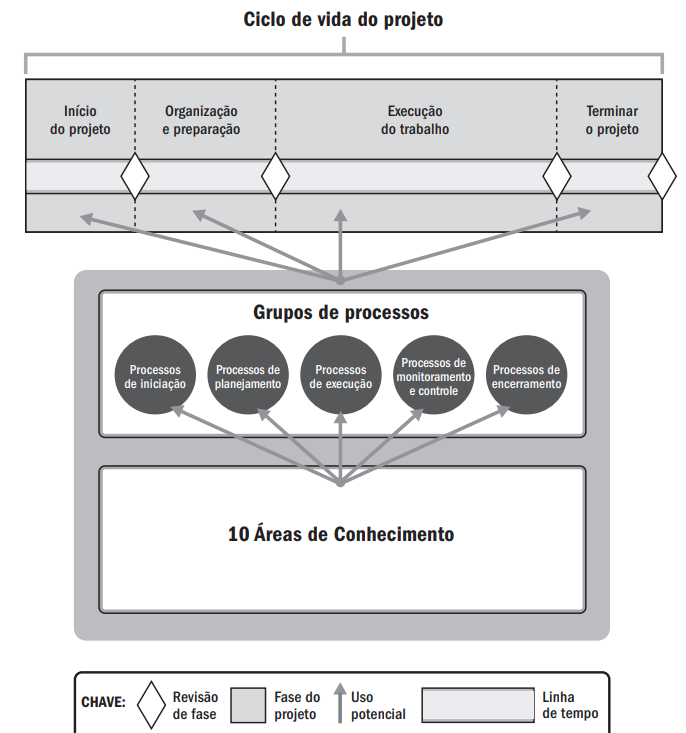
\includegraphics[scale=0.47]{src/tex/img/interrelacaoPMBOKpg18.png} \\
    \label{interrelacaoConceitos}
    \textbf{Fonte:} PMBOK \cite{PMBOK:2017}
    \centering
\end{figure}

É importante salientar que o gerenciamento de projetos na área de desenvolvimento de \textit{software} possui certas particularidades que podem trazer desafios. Como por exemplo, o fato de que os produtos desenvolvidos são intangíveis, ou seja não são tão explícitos como, por exemplo, um projeto de engenharia civil. Assim, partes inacabadas do projeto podem mais facilmente passarem despercebidas. Além disso, projetos de \textit{software} são muito distintos entre si, então até mesmo gerentes com grande experiência podem ter dificuldades em prever problemas. Mais, os processos de desenvolvimento de \textit{software} variam de organização para organização \cite{SOMMERVILLE:2011}.

O SWEBOK \cite{SWEBOK:2014} também enfatiza que existe um distanciamento entre os clientes e os processos necessários para desenvolver \textit{software}, tornando difícil que esses compreendam a complexidade do projeto. As contantes mudanças de requisitos são outra particularidade da área, que exige que o \textit{software} seja construído através de processos iterativos. Outras diferenças importantes são sobre a necessidade de se balancear criatividade e disciplina dentro do processo bem como o grau de complexidade de desenvolvimento e a exigência de constante atualização técnica das equipes.

\section{Gestão de riscos}

Em 1983, a Royal Society britânica publicou um relatório denominado \textit{"Risk assessment: a Study Group Report"}, que definiu risco como: A probabilidade de que um determinado evento adverso ocorra durante um período de tempo definido ou resulte de determinado desafio. Como na probabilidade no sentido da teoria estatística, o risco obedece a todas as leis formais das probabilidades combinatórias \cite{ADAMS:1995}. 

Já o PMBOK \cite{PMBOK:2017} inclui neste conceito a possibilidade de que riscos tenham também um efeito positivo no projeto. No guia são definidos dois tipos de risco: o risco individual do projeto e o risco geral do projeto. Para o PMBOK, o primeiro "é um evento ou condição incerta que, se ocorrer, provocará um efeito positivo ou
negativo em um ou mais objetivos do projeto.". E o risco geral do projeto " é o efeito da incerteza do projeto no seu todo, decorrente de todas as fontes de incerteza, incluindo riscos individuais, representando a exposição das partes interessadas às implicações de variações no resultado do projeto, sejam positivas ou negativas."

\citeonline{SOMMERVILLE:2011} ainda cita três categorias de risco relacionados a projetos de \textit{software}, são elas:

\begin{itemize}
    \item\textbf{Riscos de projeto:} São incertezas que podem impactar o cronograma ou os recursos do projeto.  
    \item\textbf{Riscos de produto:} Os riscos relacionados ao \textit{software} sendo desenvolvido, capazes de afetar a qualidade do produto.
    \item\textbf{Riscos de negócio:} Riscos que afetam a organização.
\end{itemize}

Essas categorias de riscos se sobrepõe, ou seja, um risco pode pertencer a uma ou mais categoria concomitantemente. \citeonline{SOMMERVILLE:2011} cita como exemplo a saída de um desenvolvedor experiente do time. Esse risco pode se enquadrar em risco de projeto, produto e também negócio. 

O motivo para isso é que quando o time perde um membro experiente é quase certo de que haverá uma queda na produtividade. Mesmo que o desenvolvedor seja substituído, o novo membro do projeto ainda levará tempo para aprender a realizar as tarefas. Então, tal risco possivelmente gerará um atraso no cronograma. Mais ainda, a saída de um colaborador experiente pode deixar uma lacuna de conhecimento no time e, assim, aumentam as chances de serem cometidos erros de programação. A perda da qualidade do \textit{software} enquadraria o risco em risco de produto. Por fim, a saída do programador pode ser um risco de negócio ao passo que a experiência do desenvolvedor pode ser crucial para o fechamento de novos contratos.

Para \citeonline{WAZLAWICK:2013}, os riscos estão presentes em todos os projetos de desenvolvimento de \textit{software} e, caso não se esteja atento a eles, os riscos podem prejudicar ou até mesmo inviabilizar um projeto. Ademais, de uma maneira genérica, é possível afirmar que negligenciar o planejamento em relação aos riscos é uma das maiores razões para o insucesso de um projeto de \textit{software}.

A partir desse contexto, a motivação para a gestão de risco se dá pelo fato de que riscos negativos (ameaças) não administrados podem gerar efeitos negativos no projeto, ou então, podem ser perdidos riscos positivos (oportunidades) não identificados. Portanto, o objetivo da gestão de risco é potencializar as oportunidades e minimizar as ameaças \cite{PMBOK:2017}.

Para obter tais benefícios a partir da gestão de riscos, \citeonline{HOPKIN:2010} destaca a importância de não apenas identificar e avaliar os riscos, mas também utilizar essas informações para tomar decisões mais embasadas e criar planos apropriados de resposta aos riscos. 

Esse processo completo foi formalizado pelo PMBOK \cite{PMBOK:2017} através da definição de sete processos de gerenciamento de riscos. São eles: Planejar o Gerenciamento de Riscos, Indentificar os Riscos, Realizar a Análise Qualitativa dos Riscos, Realizar a Análise Quantitativa dos Riscos, Planejar Respostas aos Riscos, Implementar Respostas a Riscos e Monitorar os Riscos. Cada um deles é apresentado com mais detalhes nas subseções a seguir.

\subsection{Planejar o Gerenciamento dos Riscos}

Segundo o \cite{PMBOK:2017}, o primeiro passo no processo de gerenciamento de risco é definir como serão conduzidas as atividades de gerenciamento. A definição é feita na concepção do projeto e deve estar concluída no início do projeto. Contudo, o processo pode ser revisitado caso ocorra, por exemplo, uma grande mudança no escopo do projeto.

Para a realização do Planejamento do Gerenciamento dos Riscos, o \citeonline{PMBOK:2017} prevê as seguintes entradas:

\begin{itemize}
    \item\textbf{Termo de abertura do projeto:} O documento que formaliza o início do projeto e descreve sem riqueza de detalhes os limites, requisitos e riscos do projeto.  
    \item\textbf{Plano de gerenciamento do projeto:} Para que o plano de gerenciamento de riscos seja coerente, deve-se levar em consideração os todos os planos de gerenciamento do projeto aprovados.
    \item\textbf{Documento do projeto:} O documento de projeto utilizado de entrada para essa fase pode ser o registro das partes interessadas, pois a partir desse documento é possível formalizar o papel de cada uma das partes dentro do projeto. E, assim, definir os responsáveis pelo gerenciamento de risco.
    \item\textbf{Fatores ambientais da empresa:} Fatores que podem impactar o planejamento como os limites gerais de riscos definidos pela organização.
    \item\textbf{Ativos de processos organizacionais:} Ativos que podem influenciar o processo de planejar o gerenciamento, como papéis e responsabilidades e a política organizacional de riscos.
\end{itemize}

Já as ferramentas e técnicas a serem utilizadas delimitadas pelo \citeonline{PMBOK:2017} são a \textbf{opinião especializada}, a \textbf{análise de dados} e \textbf{reuniões}. A primeira se refere ao aproveitamento da expertise de pessoas ou grupos em assuntos relacionados a gerenciamento de risco. A análise de dados trata em especial da análise das partes interessadas. E, por fim, as reuniões de início de projeto ou reuniões de planejamento podem incluir o desenvolvimento do \textbf{plano de gerenciamento de risco}.

O \textbf{plano de gerenciamento de risco} é a saída esperada dessa fase e pode incluir elementos como:

\begin{itemize}
    \item Estratégia dos riscos
    \item Metodologia
    \item Papéis e responsabilidades
    \item Financiamento
    \item Prazos
    \item Categoria dos riscos
    \item Apetite a riscos das partes interessadas
    \item Definições de probabilidade e impacto dos riscos
    \item Matriz de probabilidade e impacto
    \item Formatos de relatórios
    \item Acompanhamento
\end{itemize}

\subsection{Identificar os Riscos}

Sobre a identificação de riscos, \citeonline{PRESSMAN:2011} afirma que:

\begin{changemargin}{4cm}{0cm}
\begin{footnotesize}
A identificação do risco é uma tentativa sistemática para especificar ameaças ao plano do projeto (estimativas, cronograma, recursos etc.). Identificando os riscos conhecidos e previsíveis, o gerente de projeto dá o primeiro passo no sentido de evitá-los quando possível e controlá-los quando necessário.
\end{footnotesize}
\end{changemargin}

Assim, o objetivo desse processo é identificar os riscos individuais e fontes de risco. A partir da identificação, documenta-se as características dos riscos encontrados. Dessa forma, é possível agregar informações importantes para que a equipe do projeto possa responder adequadamente aos riscos \cite{PMBOK:2017}.

É importante destacar que a identificação de riscos é um processo iterativo e deve ocorrer ao longo do projeto. Além disso, todas as partes interessadas do projeto devem ser incentivadas a participar da identificação dos riscos \cite{PMBOK:2017}. 

Segundo \citeonline{WAZLAWICK:2013}, também é recomendável que os responsáveis pela identificação de riscos tenham acesso a um catálogo de riscos identificados em projetos semelhantes anteriores. 

Existem diversas maneiras de identificar os riscos individuais do projeto, entre elas estão o uso de \textit{checklists} predefinidos que podem ser obtidos na literatura ou na \textit{Internet}, reuniões e \textit{brainstormings} e a análise de cenários de projetos semelhantes anteriores \cite{WAZLAWICK:2013}.

O \citeonline{PMBOK:2017} também cita algumas entradas que podem ser utilizadas de apoio para a identificação de riscos, como estimativas de custo e duração, registro de lições aprendidas, requisitos, acordos e estudos acadêmicos e setoriais.

As saídas esperadas desse processo são o registro dos riscos identificados, que deve seguir um formato uniforme para garantir a clareza e compreensão dos riscos, e o relatório de riscos \cite{PMBOK:2017}. 

\subsection{Realizar a Análise Qualitativa dos Riscos}

Os riscos agora identificados precisam passar por uma análise para se determinar a importância de cada um deles, com o objetivo de determinar quais são os realmente relevantes para que sejam aplicados recursos na prevenção \cite{WAZLAWICK:2013}.

A análise \textbf{qualitativa} dos riscos é subjetiva, ou seja, baseia-se na percepção dos membros da equipe do projeto. Através dessa análise são priorizados os riscos, utilizando como parâmetro a probabilidade e o impacto da ocorrência \cite{PMBOK:2017}.

Esse processo, assim como a identificação de riscos, é iterativo e é realizado à medida que novos riscos são identificados. O objetivo desse processo é garantir que seja demandado maior esforço nos riscos considerados mais prioritários \cite{PMBOK:2017}.

Algumas ferramentas e técnicas sugeridas pelo \citeonline{PMBOK:2017} são opinião especializada, técnicas de coleta de dados como entrevistas, análise de dados, o uso de um facilitador, categorização dos riscos e reuniões.

\subsection{Realizar a Análise Quantitativa dos Riscos}

Esta análise é responsável por quantificar a exposição aos riscos do projeto e servir como uma base para o planejamento de respostas aos riscos. Dessa forma, para atingir tal objetivo, este processo realiza a análise numérica da combinação dos possíveis impactos dos riscos individuais \cite{PMBOK:2017}.

A análise quantitativa dos riscos é descrita pelo \citeonline{PMBOK:2017} tal qual um processo dispensável para certos projetos. Pois, demanda a utilização de dados de boa qualidade sobre os riscos do projeto. Assim, essa análise depende de \textit{softwares} especializados e pode consumir muitos recursos do projeto. Recomenda-se, então, que essa etapa seja utilizada em projetos mais complexos ou de grande porte. 

Algumas entradas do processo descritas pelo \citeonline{PMBOK:2017}
são o plano de gerenciamento de riscos, estimativas, relatórios e registros de riscos e estudos de projetos semelhantes. As ferramentas e técnicas que podem ser utilizadas são entrevistas, opiniões especializadas e formas de análise de dados como modelos de simulação, análise de sensibilidade e análise de árvore de decisão. 

\subsection{Planejar as Respostas aos Riscos}

O processo de Planejar as Respostas aos Riscos envolve criar estratégias para lidar com a exposição geral aos riscos e aos riscos individuais do projeto. Este processo ocorre ao longo do projeto e tem como principal objetivo minimizar os impactos negativos provenientes de riscos e maximizar oportunidades \cite{PMBOK:2017}.

Estes planos devem ser colocados em prática antes que o risco ocorra. Pode-se classificar os riscos quanto a sua exposição para que se defina quando os planos devem ser desenhados. Por exemplo, riscos de alta exposição precisam de planos definidos ainda na fase de planejamento de projeto e riscos de média exposição não necessariamente precisam ser colocados em prática de imediato, podem ser guardados e executados se a exposição aumentar \cite{WAZLAWICK:2013}.

Dessa forma, \citeonline{WAZLAWICK:2013} apresenta a seguinte tabela como uma maneira para calcular a exposição dos riscos:

\begin{flushleft}
\begin{longtable}{|p{2cm}|p{3cm}|p{3cm}|p{3cm}|p{3cm}|}
    \caption{Cálculo para exposição de um risco}
    \label{ExposicaoRisco}
    \centering
    \hline
    \multicolumn{2}{|c|}{} & \multicolumn{3}{|c|}{\cellcolor{lightgray} Probabilidade } \\ \cline{3-5}
    \multicolumn{2}{|c|}{} & Alta & Média & Baixa \\
    \hline
    \cellcolor{lightgray} Impacto & Alto & Alta exposição & Alta exposição & Média exposição \\
    \cellcolor{lightgray} & Médio & Alta exposição & Média exposição  & Baixa exposição      \\
    \cellcolor{lightgray} & Baixo & Média exposição & Baixa exposição & Baixa exposição \\
    \hline
    \addlinespace[0.2cm]
    \caption*{\textbf{Fonte:} Adaptado de \citeonline{WAZLAWICK:2013}}
\end{longtable}
\end{flushleft}

Para implementar o processo de Planejar as Respostas aos Riscos, o \citeonline{PMBOK:2017} sugere algumas estratégias. As cinco primeiras delas referem-se a riscos negativos. Sendo elas:
\begin{itemize}
    \item \textbf{Escalar: } Esta estratégia deve ser utilizada quando é determinado que a ameaça ultrapassa o escopo do projeto ou que a resposta apropriada requer uma autoridade maior que a do gerente do projeto. Assim, o risco é escalado para além do nível de projeto, podendo ser gerenciado no nível do programa, portfólio ou outra parte relevante da organização. Cabe ao gerente de projeto informar essa outra parte relevante sobre a ameaça e, a partir do momento que a parte aceitar responsabilidade sobre o risco, a equipe encerrará o monitoramento do risco.
    \item \textbf{Prevenir: } Para prevenir um risco e necessário que a equipe se empenhe para eliminá-lo ou então para evitar que tal ameaça não impacte mais o projeto. Essa estratégia é adequada para riscos de alta exposição e pode demandar que o plano de projeto seja alterado ou que o objetivo referente a esse risco seja isolado. 
    \item \textbf{Transferir: } A transferência ocorre quando se move a responsabilidade de uma ameaça a um terceiro. Esta estratégia costuma envolver o oferecimento de um prêmio ao terceiro e pode ser, por exemplo, a contratação de um seguro.
    \item \textbf{Mitigar: } Esta estratégia objetiva que os possíveis efeitos negativos do risco sejam minimizados, seja através da redução de possibilidade de ocorrência do risco ou do impacto dessa ameaça. 
    \item \textbf{Aceitar: } Ao aceitar um risco, a equipe assume a existência da ameaça porém não são adotadas ações quanto a isso. A estratégia pode ser adotada para riscos de baixa exposição ou quando não é possível tomar alguma ação, seja por impossibilidade econômica ou qualquer outro motivo.
\end{itemize}

Já para os riscos considerados positivos (oportunidades), o \citeonline{PMBOK:2017} sugere outras cinco estratégias:

\begin{itemize}
    \item \textbf{Escalar: } Da mesma forma que ameaças, as oportunidades também podem ser atribuídas a uma parte relevante da organização e não são mais monitoradas pela equipe.
    \item \textbf{Explorar: } A exploração pode ser utilizada para oportunidades que a organização deseja que sejam realizadas. Busca-se garantir que tal oportunidade de fato ocorra.
    \item \textbf{Compartilhar: } Ao adotar esta estratégia, transfere-se a responsabilidade da oportunidade a terceiros de forma que o benefício oferecido por ela seja compartilhado.   
    \item \textbf{Melhorar: } Esta estratégia busca aumentar as chances do risco positivo ocorrer ou o impacto desse, assim maximizando os benefícios obtidos. 
    \item \textbf{Aceitar: } Ao adotar esta estratégia, reconhece-se a existência da oportunidade mas não é tomada nenhuma ação quanto a ela. Assim como a aceitação de ameaças, isso pode ocorrer por impossibilidade econômica ou outros motivos.
\end{itemize}

Ao final do processo, pode ser necessário aplicar mudanças no cronograma, custos ou outros componentes do plano de gerenciamento do projeto \cite{PMBOK:2017}.

\subsection{Implementar Respostas aos Riscos}

Este processo prevê que sejam colocados os planos acordados de resposta aos riscos. Dessa forma, garante-se que aquilo que foi previamente planejado seja implementado corretamente \cite{PMBOK:2017}.

Segundo o \citeonline{PMBOK:2017}, um problema comum é o fato de que algumas equipes identificam, analisam e planejam as respostas aos riscos, mas não são tomadas providências para colocar os planos em prática. Dessa forma, este processo demanda empenho dos responsáveis pelos riscos.

\subsection{Monitorar Riscos}

O monitoramento de riscos considera a natureza volúvel e imprevisível desses. Por causa disso, é possível que ao longo do projeto novos riscos sejam descobertos, ou que a exposição dos já documentados aumente. Dessa forma, é necessário revisitar frequentemente aquilo que já foi avaliado \cite{WAZLAWICK:2013}.

Portanto, monitorar riscos é o processo de acompanhar a implementação das respostas aos riscos e também realizar novamente os outros processos, através da identificação e análise de novos riscos e elaboração de novos planos \cite{PMBOK:2017}.

Para isso, é essencial que os riscos estejam corretamente documentados \cite{WAZLAWICK:2013}, pois tanto a equipe quanto as partes interessadas devem estar a par dos riscos e níveis de exposição \cite{PMBOK:2017}. 

Assim, utiliza-se informações obtidas durante a execução do projeto para avaliar aspectos como, por exemplo, alterações nos \textit{status} dos riscos, surgimento de novos riscos ou efetividade dos planos implementados \cite{PMBOK:2017}.

O \cite{PMBOK:2017} apresenta ferramentas e técnicas para auxiliar neste processo de monitoramento. Podem ser utilizadas auditorias ou reuniões recorrentes de monitoramento de riscos. As reuniões têm como objetivo analisar e documentar se as respostas aos riscos adotadas são efetivas, além de buscar reavaliar os riscos existentes e identificar novos. A auditoria pode ser incluída como parte da reunião ou pode ser realizada de forma separada. 

O final do processo, assim como o planejamento de respostas aos riscos, pode exigir uma solicitação de mudança de custos, cronograma ou outros componentes do plano de gerenciamento do projeto \cite{PMBOK:2017}.

\section{Métodos ágeis}

Na década de 1980 e início de 1990, acreditava-se que o processo de desenvolvimento de \textit{software} deveria ser minuciosamente planejado e monitorado. Tal noção advém principalmente dos primórdios da engenharia de \textit{software}, que surgiu dentro de um contexto de \textit{softwares} robustos e duradouros como sistemas aeroespaciais e \textit{softwares} de governo. \cite{SOMMERVILLE:2011}.

Porém, esse métodos chamados de prescritivos, quando aplicados a \textit{softwares} corporativos de portes pequenos e médios, acabam prejudicando o andamento do projeto. Isso ocorre porque gasta-se mais tempo no planejamento e análise do projeto do que de fato no desenvolvimento. Além disso, tais sistemas frequentemente possuem requisitos mutáveis, o que envolve modificações no código e a adaptação das especificações. \cite{SOMMERVILLE:2011}.

\citeonline{COCKBURN:2002} argumenta que os métodos prescritivos falham ao assumir que as engenheiros de \textit{software} são máquinas. Ou seja, eles não consideram as fragilidades dos seres humanos, tais quais: diferentes estilos de trabalho, níveis de habilidades, concentração e criatividade. Além disso, erram ao assumir total disciplina e consistência por partes dos colaboradores durante um período longo de projeto.

Neste cenário de insatisfação, surgiram os métodos ágeis que possuem como principal característica a utilização de uma abordagem incremental tanto para a especificação do sistema quanto para o desenvolvimento e entrega. Assim, os métodos ágeis permitem que os \textit{softwares} sejam rapidamente entregues e facilmente adaptáveis a novos requisitos \cite{SOMMERVILLE:2011}.

A filosofia dos métodos ágeis foi descrita em 2001 por um grupo de 17 desevolvedores de \textit{software} através do Manifesto Ágil \cite{AGILEMANIFEST:2001}. Tal manifesto possui quatro valores:

\begin{itemize}
        \item Indivíduos e interações mais que processos e ferramentas;
        \item \textit{Software} em funcionamento mais que documentação abrangente;
        \item Colaboração com o cliente mais que negociação de contratos;
        \item Responder a mudanças mais que seguir um plano;
\end{itemize}

E, embora processos e ferramentas, documentação abrangente, negociação de contratos e seguir um plano sejam importantes, o manifesto valoriza mais os pontos à esquerda: Indivíduos e interações, \textit{software} em funcionamento, colaboração com o cliente e resposta à mudanças. No livro Engenharia de \textit{Software}, \citeonline{WAZLAWICK:2013} salienta que a cultura ágil não abandona planejamento, modelagem, documentação e ferramentas, ela apenas valoriza os pontos mais essenciais de um projeto de \textit{software}.

\citeonline{PRESSMAN:2011} também reforça esse ponto ao destacar que os métodos ágeis não são a antítese da engenharia de \textit{software} e sim um complemento a ser aplicado nos projetos. Ou seja, os métodos ágeis funcionam como uma filosofia para os trabalhos de \textit{software}.

Além dos quatro valores, o Manifesto Ágil \cite{AGILEMANIFEST:2001} também é composto por doze princípios: 

\begin{itemize}
        \item Nossa maior prioridade é satisfazer o cliente através da entrega contínua e adiantada de \textit{software} com valor agregado.
        \item Mudanças nos requisitos são bem-vindas, mesmo tardiamente no desenvolvimento. Processos ágeis tiram vantagem das mudanças visando vantagem competitiva para o cliente.
        \item Entregar frequentemente \textit{software} funcionando, de poucas semanas a poucos meses, com preferência à menor escala de tempo.
        \item Pessoas de negócio e desenvolvedores devem trabalhar diariamente em conjunto por todo o projeto.
        \item Construa projetos em torno de indivíduos motivados. Dê a eles o ambiente e o suporte necessário e confie neles para fazer o trabalho.
        \item O método mais eficiente e eficaz de transmitir informações para e entre uma equipe de desenvolvimento é através de conversa face a face.
        \item \textit{Software} funcionando é a medida primária de progresso.
        \item Os processos ágeis promovem desenvolvimento sustentável. Os patrocinadores, desenvolvedores e usuários devem ser capazes de manter um ritmo constante indefinidamente.
        \item Contínua atenção à excelência técnica e bom design aumenta a agilidade.
        \item Simplicidade - a arte de maximizar a quantidade de trabalho não realizado - é essencial.
        \item As melhores arquiteturas, requisitos e designs emergem de equipes auto-organizáveis.
        \item Em intervalos regulares, a equipe reflete sobre como se tornar mais eficaz e então refina e ajusta seu comportamento de acordo.
\end{itemize}

Ao refletir sobre o Manifesto Ágil \cite{AGILEMANIFEST:2001}, \citeonline{PRESSMAN:2011} define agilidade como algo que envolve, além de rápidas respostas à mudança, a entrega rápida de \textit{softwares} em funcionamento, a participação do cliente nas fases do projeto, maior facilidade de comunicação e estruturação na equipe e reconhecimento da necessidade de ser flexível quanto aos planos.

Métodos ágeis são um termo geral para uma gama de \textit{frameworks} e técnicas \cite{PMIAGILE:2017}. Portanto, cada método ágil utiliza processos distintos para instanciar os princípios da filosofia ágil demonstrados no Manifesto Ágil \cite{AGILEMANIFEST:2001}. Mesmo assim, os métodos ágeis possuem alguns pontos importantes em comum, explicitados na tabela abaixo:

\begin{longtable}{|p{5cm}|p{10cm}|}
    \caption{Princípios compartilhados pelos métodos ágeis}
    \label{tab:KeyComponents}
    \centering
            \centering
            \cr \rowcolor{lightgray}
            \textbf{Princípios} & \textbf{Descrição}
            \\ \hline
              
            \textbf{Envolvimento do cliente} &
            Os clientes devem estar intimamente envolvidos no processo de desenvolvimento. Seu papel é fornecer e priorizar novos requisitos do sistema e avaliar suas iterações.
            \\\hline
              
            \textbf{Entrega incremental} &
            0 software é desenvolvido em incrementos com o cliente, especificando os requisitos para serem incluídos em cada um.
            \\\hline
              
            \textbf{Pessoas, não processos} &
            As habilidades da equipe de desenvolvimento devem ser reconhecidas e exploradas. Membros da equipe devem desenvolver suas próprias maneiras de trabalhar, sem processos prescritivos.
            \\\hline 
              
            \textbf{Aceitar as mudanças} &
            Deve-se ter em mente que os requisitos do sistema vão mudar. Por isso, projete o sistema de maneira a acomodar essas mudanças.
            \\\hline 
              
            \textbf{Manter a simplicidade} &
            Focalize a simplicidade, tanto do software a ser desenvolvido quanto do processo de desenvolvimento. Sempre que possível, trabalhe ativamente para eliminar a complexidade do sistema.
            \\\hline
              
            \caption*{\textbf{Fonte:} Adaptado de \citeonline{SOMMERVILLE:2011}}
\end{longtable}

A Figura \ref{metodosAgeis} destaca algumas abordagens ágeis conhecidas e o compartilhamento de princípios e valores entre elas.

\begin{figure}[h]
    \centering
    \caption{Métodos ágeis}
    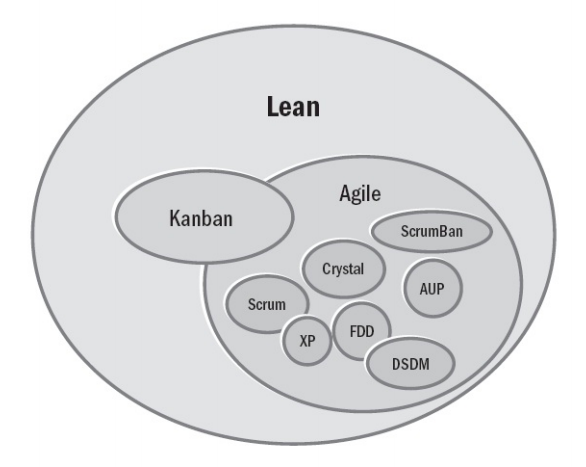
\includegraphics[scale=0.5]{src/tex/img/metodosageisPMI.png}\\
    \label{metodosAgeis}
    \textbf{Fonte:} \textit{Agile Practice Guide} \cite{PMIAGILE:2017}
\end{figure}

Nas subseções seguintes alguns dos métodos ágeis serão apresentados e elucidados.

\subsection{ \textit{Lean} }

A abordagem \textit{Lean} proposta inicialmente pela Toyota é em primeiro lugar um sistema humano e não apenas focado em cerimônias e artefatos. Ou seja, ela coloca em foco os colaborados da empresa e dá mais autonomia a eles. Essa filosofia de produção é importante para o cenário tecnológico atual ao considerar as constantes mudanças e incertezas, através da maximização do potencial humano \cite{LEANENT:2016}.

Apesar do \textit{Lean} ter sido fundamentado na indústria automobilística ele foi adaptado à indústria de software. E, nestes dias, é denominado \textit{Lean Software Development}, termo foi utilizado pela primeira vez por Tom e Mary Poppendieck \cite{WAZLAWICK:2013}.

\citeonline{Poppendieck:2006} também desenharam os princípios do \textit{Lean} para desenvolvimento de \textit{software}. São eles:

\begin{itemize}
    \item \textbf{Eliminar o desperdício:} No desenvolvimento de \textit{software} podem ser identificados diversos desperdícios, por exemplo: funcionalidades extras, levantar requisitos ou realizar testes muito cedo. Para isso, é necessário despender esforços apenas com o necessário e com o que agregue valor ao cliente.
    \item \textbf{Criar conhecimento:} Realizar ciclos de \textit{feedback}, utilizar o método científico e estimular a busca por conhecimento dentro da organização. 
    \item \textbf{Decidir tardiamente:} Ter em mente que os requisitos podem mudar e não é necessário aguardar a especificação completa para iniciar o desenvolvimento.     
    \item \textbf{Entregar o mais rápido possível:} Desenvolver \textit{software} em ciclos curtos e incrementais. E, dessa forma, garantir entregas frequentes e evitar atrasos.
    \item \textbf{Respeitar as pessoas:} Engajar e empoderar o time através de respeito mútuo e confiança.
    \item \textbf{Otimizar o todo:} Considerar o todo e não apenas as partes do \textit{software} que estão sendo desenvolvidas no momento.
    \item \textbf{Manter a qualidade:} Priorizar um código modular e incremental, evitar permanecer desenvolvendo código legado e focar nos cenários de teste.
\end{itemize}

Assim, a filosofia \textit{Lean} agrega a base para outros métodos ágeis como XP, Scrum, Kanban e Scrumban ao instaciar conceitos como foco no valor, entregas pequenas e eliminação de desperdício \cite{PMIAGILE:2017}.

\subsection{XP}

\textit{Extreme Programming} (XP) é um método utilizado desde o final da década de 80, quando teve os conceitos iniciais definidos. Porém, esse método ágil foi formalizado apenas nos anos 2000 por Kent Beck. Inicialmente, o XP era apenas aplicado em pequenas e médias equipes, porém alguns anos depois foi proposta a variação do XP, chamada \textit{Industrial XP} (IXP). Essa, por sua vez, permite a aplicação de um processo ágil em organizações de grande porte \cite{PRESSMAN:2011}. 

\citeonline{WAZLAWICK:2013} enumera os principais valores de XP da seguinte forma:

\begin{itemize}
    \item \textbf{Simplicidade:} Deve-se focar apenas nos requisitos necessários para o projeto. Ou seja, mirar em um produto simples que oferece aquilo que sabe-se que o cliente necessita.
    \item \textbf{Respeito:} O respeito deve estar presente entre os membros da equipe e também nas relações equipe-cliente. 
    \item \textbf{Coragem:} Uma equipe XP deve possuir coragem para aceitar que mudanças são inevitáveis e para acomodar essas mudanças no projeto.
\end{itemize}

Para implementar o \textit{Extreme Programming} (XP), as equipes precisam aplicar uma série de práticas baseadas nos princípios ágeis. Na figura \ref{cicloRelease} está representado um ciclo comum de entregas no XP.

\begin{figure}[h]
    \centering
    \caption{Ciclo de entregas do XP}
    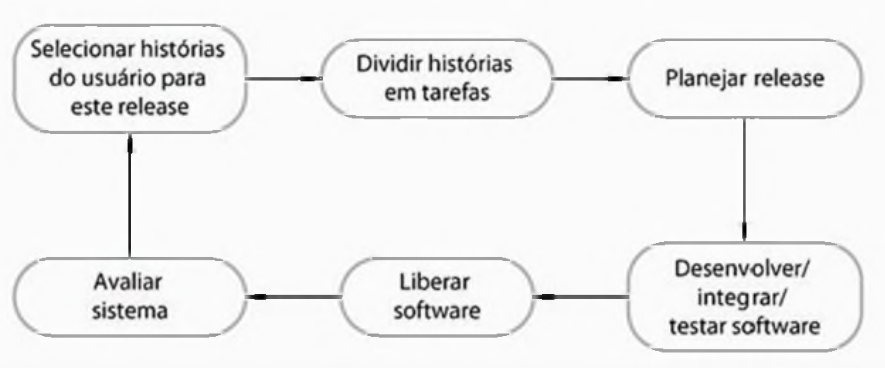
\includegraphics[scale=0.4]{src/tex/img/cicloReleaseXPSommerVille.png}\\
    \label{cicloRelease}
    \textbf{Fonte:} \citeonline{SOMMERVILLE:2011}
\end{figure}

As práticas necessárias para concluir um ciclo de \textit{release} do XP envolvem atividades desde o planejamento até especificações de como a equipe deve interagir. A primeira delas é o planejamento incremental, na qual se utiliza as histórias de usuário divididas em tarefas para realizar o planejamento de cada \textit{release}. É importante destacar que essas entregas devem ser pequenas, contínuas e contendo apenas o conjunto mínimo de funcionalidades úteis e isso reflete no princípio de que o projeto deve ser simples e apenas contemplar as atuais necessidades do cliente \cite{SOMMERVILLE:2011}.

Outra prática é o Desenvolvimento Orientado a Testes (TDD), ou seja, implementar primeiramente os testes automatizados e, após, a funcionalidade em si. No XP também é essencial que o código seja constantemente refatorado e melhorado. Esse método ágil também prevê a programação em pares (\textit{pair programming}), neste cenário os desenvolvedores trabalham em duplas, o que facilita a troca de conhecimento \cite{SOMMERVILLE:2011}.

No XP, o código deve ser de posse coletiva e, dessa forma, estabelece que esse pode ser modificado por qualquer membro da equipe sem a necessidade de permissão. Além disso, o desenvolvimento deve manter um ritmo sustentável, sem a exigência de muitas horas extras, que podem prejudicar a qualidade do produto. E, por fim, o XP considera o cliente como parte da equipe e ele deve estar disponível para diminuir possíveis barreiras de comunicação \cite{WAZLAWICK:2013}.

\subsection{\textit{Scrum}}
As bases do método ágil \textit{Scrum} foram definidas em 1986 a partir do artigo: "\textit{The New New Product Development Game} de \citeonline{Takeuchi:1986}. Esse artigo ilustrava o modelo de produção de automóveis da Honda que demonstrava algumas influências da filosofia \textit{Lean} \cite{WAZLAWICK:2013}.

Na área de desenvolvimento de \textit{software}, \textit{Scrum} é um \textit{framework} ágil formalizado por \citeonline{Sutherland:2013} através do "Um guia definitivo para o \textit{Scrum}: As regras do jogo". O nome do método tem origem em um termo de rúgbi e é um momento onde os jogadores se unem aos companheiros de time e trabalham em equipe para empurrar a bola em direção ao fundo do campo \cite{PRESSMAN:2011}. 

Segundo o Guia do \textit{Scrum} \cite{Sutherland:2013}, "o \textit{framework} \textit{Scrum} consiste nos times do Scrum associadas a papéis, eventos, artefatos e
regras." E, a partir desse \textit{framework}, as equipes podem resolver problemas complexos e adaptativos, ao mesmo tempo que garantem uma entrega de alto valor. 

Os papéis do time de \textit{Scrum} são: \textit{Scrum master} (mestre de \textit{Scrum}), \textit{product owner} (dono do produto) e \textit{development team} (equipe de desenvolvimento). O primeiro papel representa um membro da equipe com bastante conhecimento na aplicação do \textit{Scrum}. Apesar de representar um papel de lideranças, o \textit{Scrum} master não atua tal qual um gerente, ele age como um facilitador para aproximar a equipe das regras do \textit{Scrum} \cite{WAZLAWICK:2013}.

Já o \textit{product owner}, é o membro da equipe responsável pelo projeto e é quem define as funcionalidades a serem desenvolvidos a cada \textit{sprint}. Esse papel tem como objetivo identificar as necessidades do cliente e aplicá-las da maneira menos custosa possível. Por fim, o \textit{development team} são os membros que de fato desenvolvem o projeto, sem distinção entre papéis como desenvolvedores, analistas, \textit{designers} e testadores \cite{WAZLAWICK:2013}.

\citeonline{PRESSMAN:2011} destaca que o \textit{Scrum} utiliza um conjunto de padrões de processo que define um conjunto de ações de desenvolvimento. Esses padrões estão representados na Tabela abaixo e divididos em dois grupos: Eventos e Artefatos.

\begin{longtable}{|c|c|}
    \caption{Eventos e Artefatos do \textit{Scrum}}
    \label{tab:KeyComponents}
    \centering
              \centering
              \cr \rowcolor{lightgray}

            \textbf{Eventos} & \textbf{Artefatos} \\
            \hline 
            \textit{Sprint} & \textit{Product backlog}\\

            \textit{Sprint planning} & \textit{Sprint backlog}\\

            \textit{Daily scrum} & Incrementos\\

            \textit{Sprint review} & \\

            \textit{Sprint retrospective} & \\ \hline
            \addlinespace[0.2cm]
            \caption*{\textbf{Fonte:} Adaptado de \citeonline{PMIAGILE:2017}}
\end{longtable}

Os \textit{backlogs} são o registro de trabalhos pendentes. Consiste em uma lista priorizada com os requisitos a serem cumpridos \cite{PRESSMAN:2011}. O \textit{product backlog} costuma possuir histórias de usuário com uma descrição simples, um identificador e prioridade. Enquanto o \textit{sprint backlog} contém o plano daquela iteração corrente e já com os requisitos detalhados em formas de tarefas para as equipes de desenvolvimento realizarem. E, os incrementos são todo o trabalho realizado no período de uma \textit{sprint} \cite{WAZLAWICK:2013}.

As \textit{sprints} recebem esse nome por serem associadas à corridas de curta distância. Elas consistem em uma janela de tempo em que os trabalhos do \textit{sprint backlog} devem ser desenvolvidos. Elas ocorrem em forma de iterações, ao término o \textit{sprint backlog} é ajustado \cite{PRESSMAN:2011}.

Tratando agora das cerimônias do \textit{Scrum}, no começo de cada nova \textit{sprint} é feito o \textit{Sprint planning}, uma reunião na qual a equipe seleciona os elementos do \textit{product backlog} a serem desenvolvidos naquele ciclo. Essa reunião responde as perguntas: "O que pode ser entregue como resultado do incremento da próxima Sprint?" e "Como o trabalho necessário para entregar o incremento será realizado?" \cite{Sutherland:2013}.

A \textit{Daily scrum} é uma reunião diária que tem como o objetivo inspecionar o trabalho desenvolvido pela equipe desde a última \textit{Daily scrum} e também identificar obstáculos que estejam impedindo o progresso do time de desenvolvimento \cite{Sutherland:2013}. 

A \textit{Sprint review} e \textit{Sprint retrospective} devem ocorrer ao final de cada \textit{sprint}. A primeira, trata-se de uma avaliação do produto desenvolvido durante a \textit{sprint} e onde é feita a validação dos requisitos. Já a \textit{Sprint retrospective} trata da avaliação do processo de desenvolvimento e da equipe. A equipe, então, reflete sobre o passado e discute aquilo que deu certo e aquilo que precisa ser melhorado \cite{WAZLAWICK:2013}.

\subsection{Kanban}

Kanban é um nome de origem japonesa que significa "sinal" ou "cartão" e surgiu dos sistemas de cartão utilizados para gerenciar o fluxo de trabalho em indústrias. Assim, o principal objetivo desse sistema é tornar o andamento do trabalho visível a todos os membros da equipe \cite{Mariotti:2012}. Esse modelo foi adaptado da indústria para o desenvolvimento de \textit{software} por David J. Anderson \cite{Ghisi:2012}. 

As atividades essenciais para a implementação do Kanban consistem em: visualizar, limitar o trabalho em progresso, gerenciar o fluxo \cite{Mariotti:2012}. 

Para a primeira atividade listada, faz-se uso do quadro kanban. O quadro num geral possui colunas que representam os passos do processo para diferenciar o estado atual de cada um dos cartões. Esses cartões descrevem itens de trabalho e destacam visualmente as tarefas a serem desenvolvidas \cite{ANDERSON:2016}. A Figura \ref{fig:kanban} apresenta uma possível representação de um quadro kanban.

\begin{figure}[h!]
    \centering
    \caption{Quadro kanban}
    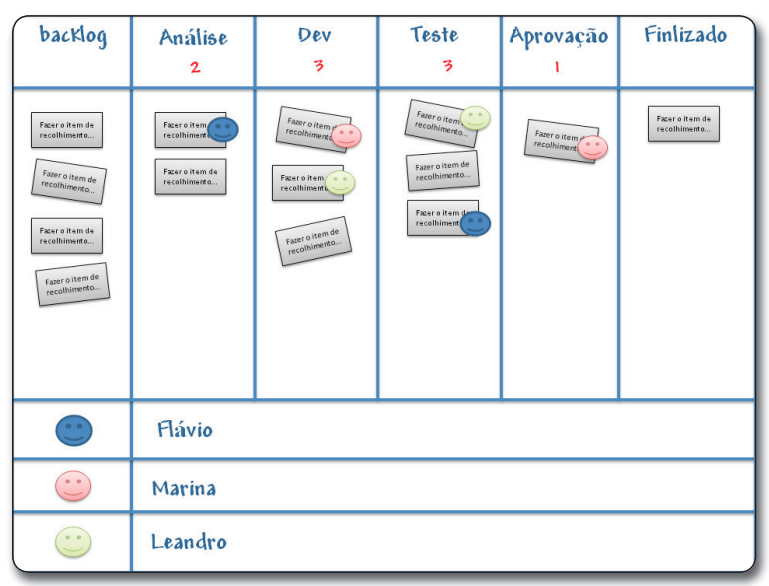
\includegraphics[width=0.8\textwidth]{src/tex/img/quadroKanban.png}\\
    \textbf{Fonte:} \citeonline{Mariotti:2012}
    \label{fig:kanban}
\end{figure}

Outra atividade é limitar o trabalho em progresso, do inglês WIP (\textit{work in progress}) \cite{Mariotti:2012}. Esta atividade considera que deve-se apenas começar novas tarefas quando o trabalho atual for concluído. Isso evita que a equipe acabe com muitas tarefas incompletas em mãos. Assim, o Kanban considera que é essencial que o WIP não possa ultrapassar o valor determinado pela equipe \cite{ANDERSON:2016}.

O controle de fluxo leva em conta o \textit{lead time}, que corresponde ao tempo em que determinada tarefa leva para passar por todas as colunas até a entrega \cite{Mariotti:2012}. Assim, o gerenciamento do \textit{lead time} busca minimizar gargalos e tempo de espera, enquanto se maximiza a entrega de valor \cite{ANDERSON:2016}. 

\section{Guia para gestão ágil de riscos}

O Guia para gestão ágil de riscos foi desenvolvido no contexto do Grupo de Qualidade de Software da Universidade Federal de Santa Catarina (UFSC) em 2020. O trabalho foi elaborado como parte de sua monografia para conclusão de curso de um estudante de Sistemas de Informação da UFSC.

O guia contém práticas de gerenciamento ágil de riscos, tendo sido criado com foco em organizações que desenvolvem \textit{software} e utilizou como base a literatura, o estado da arte e a experiência dos autores \cite{Vieira:2020}.

Segundo \citeonline{Vieira:2020}, o guia apresenta os seguintes elementos em sua estrutura:

\begin{itemize}
    \item \textbf{Papéis: } Os papéis envolvidos na realização das tarefas presentes nas atividades para gerenciamento de risco.
    \item \textbf{Cerimônias: } As cerimônias apresentadas pelo guia são reuniões com diferentes periodicidades e características. Estas reuniões preveem a participação de diversos papéis e são utilizadas para discussões sobre o projeto. 
    \item \textbf{Atividades: } Apresentam ações com objetivos pré-determinados, podendo ser realizadas de forma agrupada ou individual.
    \item \textbf{Tarefas: } As tarefas estabelecem passos para se atingir um objetivo pré-determinado. As atividades podem ser compostas de uma ou mais tarefas. 
    \item \textbf{Técnicas: } Os conjuntos de passos implementados pelas tarefas. As técnicas podem ser reutilizadas, diferentemente das tarefas que são únicas.
    \item \textbf{Produtos de Trabalho: } As atividades, tarefas e técnicas resultam em produtos de trabalho, que permitem a avaliação quantitativa ou qualitativa do trabalho realizado.  
    \item \textbf{Ferramentas: } As ferramentas são os recursos utilizados no desenvolvimento de uma tarefa. Essas podem ser físicas ou virtuais e fundamentais ou opcionais.
\end{itemize}

\begin{figure}
    \centering
    \caption{Estrutura padrão do Guia de gestão ágil de riscos.}
    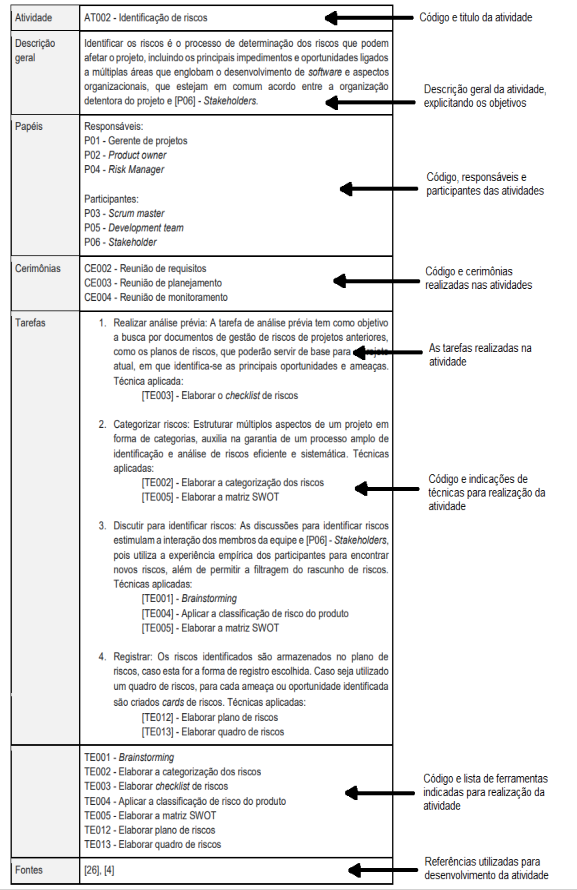
\includegraphics[width=\textwidth,height=\textheight,keepaspectratio]{src/tex/img/estrutura-guia.png}
    \textbf{Fonte:} \citeonline{Vieira:2020}
    \label{fig:my_label}
\end{figure}

Mesmo contendo práticas de gestão de riscos da literatura e das organizações que desenvolvem \textit{software} e ter sido avaliado por um painel de especialistas, o guia não chegou a ser avaliado na prática. Assim, são necessários resultados de sua aplicação empírica para validar as práticas documentadas.

\chapter{Estado da arte}
\label{sec:EstadoArte}

O objetivo deste capítulo é apresentar o estado da arte do tema proposto por este trabalho. Para isso, foi realizado um Mapeamento Sistemático da Literatura (MSL) em conjunto com o trabalho de mestrado do aluno Fernando Vedoin Garcia \cite{GARCIA:2021}. A MSL foi desenvolvida com base nas etapas propostas por \citeonline{Kitchenham:2004} no relatório "\textit{Procedures for performing systematic reviews}". 

O foco principal desta Revisão Sistemática da Literatura é identificar e analisar os atuais estudos empíricos sobre a aplicação de técnicas de gestão de riscos em contextos de desenvolvimento ágil. Levando em consideração quais técnicas foram aplicadas e os resultados obtidos a partir da aplicação.

\section{Mapeamento Sistemático da Literatura}

A realização da MSL utilizou as três etapas definidas por \citeonline{Kitchenham:2004}, identificadas abaixo: 

\begin{enumerate}
    \item Planejamento da revisão
        \begin{enumerate}
            \item Identificação da necessidade da revisão
            \item Desenvolvimento do protocolo de busca
        \end{enumerate}
    \item Condução da revisão
        \begin{enumerate}
            \item Identificação da pesquisa
            \item Seleção dos estudos primários
            \item Avaliação da qualidade dos estudos
            \item Extração de dados e monitoramento
            \item Sintetização dos dados
        \end{enumerate}
    \item Relatório da MSL
\end{enumerate}

\section{Definição do Protocolo de Revisão}

Com base nos objetivos da pesquisa identificada para este trabalho, foi definida a seguinte questão geral de pesquisa: "Quais são os resultados dos estudos empíricos de gestão de riscos em métodos ágeis?".

Após, foi utilizada a metodologia PICOC, sigla de População, Intervenção, Comparação, \textit{Outcome} (Resultado) e Contexto derivada da estratégia PICO utilizada na área médica \cite{SANTOS:2007}. Assim, foram definidos os seguintes elementos:

\begin{longtable}{|c|p{10cm}|}
    \caption{Descrição dos elementos PICOC}
    \label{tab:PICOCElements}
    \centering
              \centering
              \cr \rowcolor{lightgray}

            \textbf{Critérios} & \textbf{Descrição} 
            \\\hline 
            
            População & Organizações de \textit{software}.
            \\\hline
            
            Intervenção & Aplicação de técnicas de gerência de risco no contexto da organização.
            \\\hline

            Comparação & N/A
            \\\hline

            Resultado & Analisar se o processo e as características gerais do projeto foram impactadas.
            \\\hline

            Contexto & Utilização de métodos ágeis.
            \\\hline
            \addlinespace[0.2cm]
            \caption*{\textbf{Fonte:} Desenvolvido pela autora (2021).}
\end{longtable}

A partir da identificação dos elementos da Tabela \ref{tab:PICOCElements}, foram levantadas as seguintes questões de pesquisa: 

\begin{itemize} [label={}]
    \item \textbf{Q1.} Quais são os estudos que tratam de integração de práticas de gestão de riscos nos métodos ágeis?
    \item \textbf{Q2.} Qual contexto de uso de práticas de gestão de riscos nos métodos ágeis?
    \item \textbf{Q3.} Quais as características do ambiente de aplicação?
    \item \textbf{Q4.} Qual a motivação para a introdução de práticas explícitas de gestão de riscos nos métodos ágeis?
    \item \textbf{Q5.} Quais práticas de gestão de riscos são introduzidas nos métodos ágeis?
    \item \textbf{Q6.} Quais riscos são gerenciados?
    \item \textbf{Q7.} Quais os resultados da introdução de práticas explícitas de gestão de riscos nos métodos ágeis?
\end{itemize}

\section{Bases de dados}

\citeonline{Kitchenham:2004} destaca a importância do uso de bases de dados digitais para a área de Engenharia de \textit{Software}. Por isso, foram selecionadas três bibliotecas e bases de dados digitais relevantes para a área deste trabalho, são elas: ACM Digital Library, IEEExplore e Scopus. 

\section{Critérios de pesquisa}

Após a seleção das bases de dados, foram determinados critérios de busca para a seleção de artigos. Segundo \citeonline{Kitchenham:2004}, os estudos devem passar por uma série de estágios para serem escolhidos. O primeiro deles é aplicar os critérios de elegibilidade, após, filtra-se pelos títulos e resumos. Por fim, os trabalhos que não forem excluídos são analisados mais detalhadamente. Os critérios utilizados para realizar o primeiro filtro dos trabalhos foram:

\begin{itemize}
    \item Critérios de inclusão
        \begin{itemize}
            \item Estudos primários publicados que passaram por revisão por pares.            \item Estudos em Inglês ou Português.
            \item Artigos completos (mínimo 4 páginas).
            \item Estudos publicados até o ano de 2021.
        \end{itemize}
    \item Critérios de exclusão
        \begin{itemize}
            \item Estudos teóricos, não empíricos.
            \item Estudos duplicados.
            \item Estudos que não estejam acessíveis pela rede da Universidade Federal de Santa Catarina (UFSC).
            \item Estudos sem foco principal em desenvolvimento de \textit{software}.
        \end{itemize}
\end{itemize}


\section{Termos de pesquisa}

Foram selecionados, então, os termos de buscas mais relevantes para o tema deste trabalho. A Tabela \ref{tab:ResearchTerms} apresenta os termos utilizados para refinar as buscas nas bases de dados e seus respectivos sinônimos. Entre eles estão \textit{software}, \textit{Risk management} e \textit{agile}. Os termos foram extraídos a partir de alguns elementos do PICOC. \\ \\

\begin{longtable}{|p{2.5cm}|p{4cm}|p{8cm}|}
    \caption{Termos de busca}
    \label{tab:ResearchTerms}
    \centering
              \centering
              \cr \rowcolor{lightgray}
            \textbf{Critério} & \textbf{Termo} & \textbf{Sinônimos} 
            \\ \hline 
            
            \textbf{População} & \textit{Software} & N/A
            \\ \hline

            \textbf{Invervenção} & \textit{Risk Management} & \textit{Risk analysis, Risk administration, Management of risk}
            \\ \hline

            \textbf{Contexto} & \textit{Agile} & \textit{Scrum}, XP, \textit{Extreme Programming}, \textit{Lean}, Kanban, FDD, \textit{Feature Driven Development}, \textit{Crystal}, \textit{Iterative Development}
            \\ \hline 
            \addlinespace[0.2cm]
            \caption*{\textbf{Fonte:} Desenvolvido pela autora (2021).}
\end{longtable}

\section{\textit{Strings} de busca}

As \textit{strings} de busca sofreram adaptações para que retornassem resultados relacionados ao tema do presente trabalho. Na Tabela \ref{tab:StringsBusca} são apresentadas as \textit{strings} de busca utilizadas para cada base de dados.

\begin{longtable}{|c|p{11cm}|}
    \caption{\textit{Strings} de busca}
    \label{tab:StringsBusca}
    \centering
              \centering
              \cr \rowcolor{lightgray}

            \textbf{Base de dados} & \textbf{\textit{Strings} adaptadas} 
            \\ \hline 
            
            ACM Digital Library & (Abstract:(risk) AND Abstract:(agile OR scrum OR xp OR "extreme programming" OR lean OR kanban OR scrumban OR fdd OR "feature driven development" OR  Crystal OR "Iterative Development")) OR (Title:(risk) AND Title:(agile OR scrum OR xp OR "extreme programming" OR lean OR kanban OR scrumban OR fdd OR "feature driven development" OR  Crystal OR "Iterative Development"))
            \\ \hline
            
            IEEEXplore & All Metadata":risk AND ("All Metadata":agile OR "All Metadata":scrum OR "All Metadata":xp OR "All Metadata":"extreme programming" OR "All Metadata":lean OR "All Metadata":kanban OR "All Metadata":scrumban OR "All Metadata":fdd OR "All Metadata":“feature driven development” OR "All Metadata":Crystal OR "All Metadata":"Iterative Development")
            \\ \hline

            Scopus & (TITLE-ABS-KEY (risk) AND (TITLE-ABS-KEY(agile) OR TITLE-ABS-KEY (scrum) OR TITLE-ABS-KEY (xp) OR TITLE-ABS-KEY (extreme AND programming) OR TITLE-ABS-KEY (lean) OR TITLE-ABS-KEY (kanban) OR TITLE-ABS-KEY (scrumban) OR TITLE-ABS-KEY (fdd) OR TITLE-ABS-KEY (feature AND driven AND development) OR TITLE-ABS-KEY (crystal) OR TITLE-ABS-KEY (iterative AND development)) AND (LIMIT-TO (SUBJAREA,"COMP")))
            \\ \hline

            \addlinespace[0.2cm]
            \caption*{\textbf{Fonte:} Desenvolvido pela autora (2021).}
\end{longtable}

As bases de dados retornaram no total 2815 estudos após a aplicação das \textit{strings}. E, os estudos foram distribuídos conforme a Figura \ref{EstudosRetornados}.

\begin{figure}[h]
    \centering
    \caption{Estudos retornados em cada base de dados}
    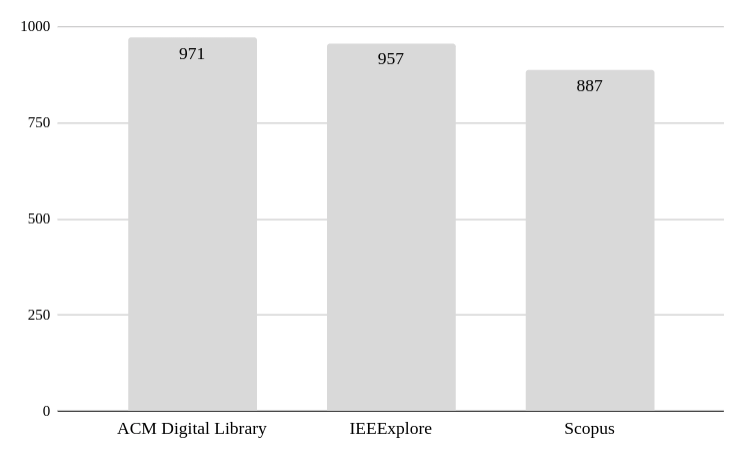
\includegraphics[scale=0.55]{src/tex/img/graficoBuscas.png} \\
    \label{EstudosRetornados}
    \textbf{Fonte:} Desenvolvido pela autora (2022).
    \centering
\end{figure}

\section{Seleção dos artigos}

Mesmo com as \textit{strings} de busca limitando o conteúdo dos estudos retornados, ainda assim as buscas resultaram em um volume grande de estudos. Por isso, foi realizada uma filtragem através da leitura dos títulos.

A partir dos artigos restantes, fez-se uma segunda filtragem que teve como critério a leitura dos resumos e a estrutura geral dos artigos. Desta forma, foi possível aplicar os critérios de inclusão, exclusão e qualidade para cada um deles. 

Enfim, após a segunda filtragem, foi realizada a leitura integral do texto de cada trabalho. Com base nesta leitura, foi possível identificar aqueles mais relevantes com base nas perguntas de pesquisa. Esses, então, foram selecionados para a extração e análise dos dados. A figura abaixo demonstra a distribuição dos artigos selecionados por ano de publicação:

\begin{figure}[h]
    \centering
    \caption{Artigos por ano de publicação}
    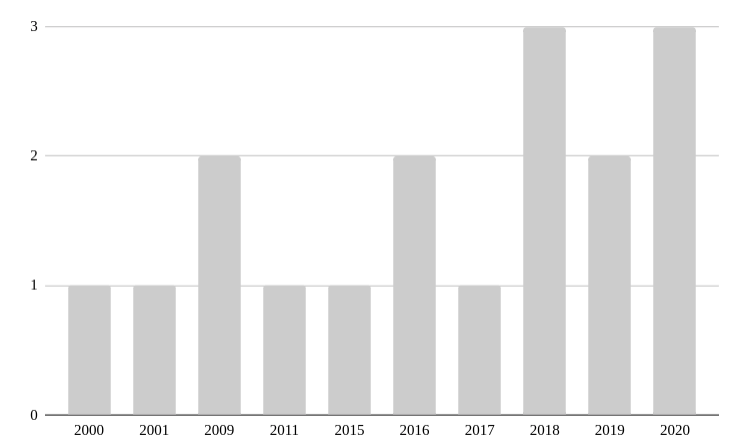
\includegraphics[scale=0.55]{src/tex/img/artigosAno.png} \\
    \label{EstudosRetornados}
    \textbf{Fonte:} Desenvolvido pela autora (2022).
    \centering
\end{figure}

\section{Extração de dados}

Para realizar a coleta de dados, foram selecionados dados relevantes a serem levantados nos artigos com base nas perguntas de pesquisa. A partir de tais dados, foram criadas questões de análise. As questões foram definidas segundo a Tabela \ref{tab:QAnalise}.

\begin{longtable}{|p{8cm}|p{5cm}|}
    \caption{Questões de análise}
    \label{tab:QAnalise}
    \centering
            \centering
            \cr \rowcolor{lightgray}
            \textbf{Questão de pesquisa} & \textbf{Questões de análise} 
            \\ \hline 
            
            \multirow{1}{12em}{\textbf{Q2.} Qual contexto de uso de práticas de gestão de riscos nos métodos ágeis?}
            & \textbf{Q2.1} Contexto de uso \\
            & \textbf{Q2.2} Método Ágil \\
            & \textbf{Q2.3} Tipo do estudo \\
            & \textbf{Q2.4} Quantidade de organizações
            \\ \hline
            
            \multirow{1}{12em}{\textbf{Q3.} Quais as características do ambiente de aplicação?}
            & \textbf{Q3.1} Tamanho da equipe \\
            & \textbf{Q3.2} Domínio da aplicação \\
            & \textbf{Q3.3} Tamanho do produto \\
            & \textbf{Q3.4} Duração do projeto
            \\ \hline
            
            \multirow{1}{12em}{\textbf{Q4.} Qual a motivação para a introdução de práticas explícitas de gestão de riscos nos métodos ágeis?}
            & \textbf{Q4.1} Lista de motivos \\ & \\ & \\ &
            \\ \hline
            
            \multirow{1}{12em}{\textbf{Q5.} Quais práticas de gestão de riscos são introduzidas nos métodos ágeis?}
            & \textbf{Q5.1} Lista de práticas \\ & \\ & \\ &
            \\ \hline
            
            \multirow{1}{12em}{\textbf{Q6.} Quais riscos são gerenciados?}
            & \textbf{Q6.1} Lista de riscos \\ & 
            \\ \hline
            
            \multirow{1}{12em}{\textbf{Q7.} Quais os resultados da introdução de práticas explícitas de gestão de riscos nos métodos ágeis?}
            & \textbf{Q7.1} Lista de resultados \\ & \\ & \\ &
            \\ \hline
            \addlinespace[0.2cm]
            \caption*{\textbf{Fonte:} Desenvolvido pela autora (2021).}
\end{longtable}

\section{Análise dos resultados}

Nesta seção foi realizada a síntese e classificação dos estudos selecionados, estes estão numerados e referenciados no Apêndice \ref{sec:ApendiceA}.

\textbf{Q1. Quais são os estudos que tratam de integração de práticas de gestão de riscos nos métodos ágeis?}

Como resultado do MSL, foram encontrados os estudos listados no Apêndice \ref{sec:ApendiceA} que tratam da integração das práticas de gestão de riscos nos métodos ágeis.

\textbf{Q2. Qual contexto de uso de práticas de gestão de riscos nos métodos ágeis?}

O contexto de uso se refere ao tipo de ambiente de aplicação (Q2.1), método ágil adotado (Q2.2), tipo de estudo (Q2.3) e quantidade de organizações participantes (Q2.4).

Um dos critérios de exclusão era o de estudos teóricos, assim, todos os estudos selecionados são empíricos, ou seja, foram aplicados. A aplicação de cada trabalho ocorreu em um desses dois ambientes: academia e indústria de \textit{software}. Assim, 13 dos estudos selecionados (76\%) foram aplicados em organizações de desenvolvimento de \textit{software} enquanto 4 (24\%) foram aplicados em um ambiente acadêmico em que alunos avaliaram o modelo, ferramentas ou conjuntos de práticas. 

A maioria dos estudos (13) foram aplicados em apenas uma organização. Enquanto o [17] foi validado em 5 diferentes organizações, com características distintas de tamanho, complexidade e processo de desenvolvimento.

Quanto aos métodos ágeis adotados por cada uma das organizações participantes dos estudos, 8 (47\%) adotaram Scrum, 3 (18\%) adotaram XP, 2 (12\%) adotaram Kanban e apenas o [10] citou o Dynamic System Development Method (DSDM). Porém, dos trabalhos selecionados 7 (58\%) não especificaram um método ágil.

Sobre o tipo de estudo empírico, a maioria (14) aplicaram um estudo de caso, representando 82\% do total dos estudos selecionados. Enquanto 2 (12\%) aplicaram experimentos e apenas o [8] aplicou uma prova de conceito. O estudo de caso foi o tipo de estudo mais utilizado na indústria, enquanto na academia houve um equilíbrio entre as técnicas. 

\begin{longtable}{|p{4cm}|p{4cm}|p{8cm}|}
    \caption{Extração dos dados - Contexto}
    \label{tab:ContextoEstudos}
    \centering
             \centering
             \cr \rowcolor{lightgray}
            \multicolumn{2}{|c|}{\textbf{Classificação}} & \textbf{Estudos} 
            \\ \hline 
            
            \multirow{1}{10em}{\textbf{Q2.1} Contexto de uso}
            & Indústria & [1], [2], [4], [5], [8], [10], [11], [12], [13], [14], [15], [16], [17] \\ 
            & Academia & [3], [6], [7], [9]
            \\ \hline
            
            \multirow{1}{10em}{\textbf{Q2.2} Métodos ágeis utilizados no estudo}
            & \textit{Scrum} & [2], [5], [6], [7], [9], [10], [12], [14] \\ 
            & Kanban & [8], [14] \\ 
            & XP & [10], [11], [14] \\
            & DSDM & [10] \\
            & Não informado & [1], [3], [4], [13], [15], [16], [17]
            \\ \hline
            
            \multirow{1}{10em}{\textbf{Q2.3} Tipo do estudo}
            & Experimento & [3], [9] \\ 
            & Estudo de caso & [1], [2], [4], [5], [6], [7], [10], [11], [12], [13], [14], [15], [16], [17] \\ 
            & Prova de conceito & [8] 
            \\ \hline
            
            \multirow{1}{10em}{\textbf{Q2.4} Quantidade de organizações}
            & 1 &  [1], [2], [4], [5], [6], [7], [8], [11], [12], [13], [14], [15], [16] \\ 
            & Entre 2 e 10 & [10], [17] \\ 
            & Não informado & [3], [9]
            \\ \hline
            
            \addlinespace[0.2cm]
            \caption*{\textbf{Fonte:} Desenvolvido pela autora (2021).}
            \end{longtable}
            
\textbf{Q3. Quais as características do ambiente de aplicação?}

Para desenhar as características do ambiente de aplicação, foram utilizados os seguintes parâmetros: tamanho da equipe (Q3.1), domínio de aplicação (Q3.2), tamanho do produto (Q3.3) e duração do projeto (Q3.4).

Em média, o tamanho das equipes permaneceu equilibrado entre os estudos, com maior concentração entre 6 e 10 membros. O estudo com o menor número de membros na equipe é o [7], com apenas 4 membros. Outro destaque é o estudo [7] que foi aplicado em um ambiente com 320 pessoas alocadas em 20 projetos diferentes. Neste caso, foi considerada uma média de 16 membros por equipe.

Foram definidos três tamanhos para os produtos desenvolvidos pelas organizações: grande, pequeno ou não informado. Dos estudos selecionados, 10 (59\%) dos trabalhos desenvolvidos foram classificados como grande. Indicando que projetos maiores utilizam os métodos ágeis, mesmo os projetos maiores necessitando de maior atenção quanto à gestão de risco.

Sobre o domínio da aplicação, essa foi a característica com maior variabilidade entre os ambientes. Um exemplo é o estudo [10], neste estudo a aplicação se deu em 10 projetos distintos que variavam entre as áreas de \textit{e-learning}, mobilidade, gestão de hotéis, \textit{e-commerce}, gestão de biblioteca, \textit{internet banking}, governo, saúde, construção e militar. Os domínios de aplicação de cada um dos estudos está descrito na Tabela \ref{tab:AmbienteEstudos}.

Além disso, apenas 29\% dos estudos descreviam a duração do projeto. Esta informação também está disponível na Tabela \ref{tab:AmbienteEstudos}.

\begin{longtable}{|p{4cm}|p{4cm}|p{8cm}|}
    \caption{Extração dos dados - Ambiente}
    \label{tab:AmbienteEstudos}
    \centering
             \centering
             \cr \rowcolor{lightgray}
            \multicolumn{2}{|c|}{\textbf{Classificação}} & \textbf{Estudos} 
            \\ \hline 
            
            \multirow{1}{10em}{\textbf{Q3.1} Tamanho da equipe}
            & Entre 1 e 5 & [2], [4], [6], [7]\\ 
            & Entre 6 e 10 &  [2], [5], [6], [11]\\ 
            & Mais de 10 & [4], [5] \\
            & Não informado & [1], [3], [8], [9], [10], [12], [13], [14], [15], [16], [17]
            \\ \hline
            
            \multirow{1}{10em}{\textbf{Q3.2} Domínio da aplicação}
            & ETL & [14]\\
            & Telecomunicações & [12], [15]\\
            & Mobilidade & [10], [14]\\
            & Militar & [1], [10]\\
            & Financeiro & [2], [12], [16]\\
            & E-commerce & [4], [7], [8], [10]\\
            & E-learning & [10]\\
            & Gestão & [10], [11], [14]\\
            & Internet Banking & [10]\\
            & Saúde & [10], [13], [14]\\
            & Construção & [10], [12]\\
            & Governo & [10]\\
            & Não definido & [3], [5], [6], [9], [17]
            \\ \hline
            
            \multirow{1}{10em}{\textbf{Q3.3} Tamanho do produto}
            & Grande & [1], [2], [4], [8], [10], [13], [14], [15], [16], [17] \\ 
            & Pequeno & [6], [7] \\ 
            & Não informado & [3], [5], [9], [11], [12]
            \\ \hline
            
            \multirow{1}{10em}{\textbf{Q3.4} Duração do projeto}
            & Entre 1 e 3 meses & [5], [7], [12]\\
            & Entre 4 e 6 meses & [2]\\
            & Mais de 6 meses & [15]\\
            & Não informado & [1], [3], [4], [8], [9], [10], [11], [13], [14], [16], [17]
            \\ \hline
        
            \addlinespace[0.2cm]
            \caption*{\textbf{Fonte:} Desenvolvido pela autora (2022).}
\end{longtable}

\textbf{Q4. Qual a motivação para a introdução de práticas explícitas de gestão de riscos nos métodos ágeis?}

O principal motivo descrito pelos estudos foi que as práticas ágeis de gerenciamento de risco não são suficientes para suprir essa demanda. Assim, existe a necessidade da gestão explícita de riscos com práticas definidas para incrementar os métodos ágeis. Este motivo foi citado por 4 estudos (24\%), sendo eles os estudos [3], [4], [5] e [9].

Contudo, os estudos [6] e [17] listaram 3 motivos pelos quais a gestão de riscos deve complementar os métodos ágeis. O estudo [6] destacou que não existe um processo e/ou ferramenta para gestão de risco comumente utilizado na área de desenvolvimento de \textit{software}. Além disso, salientou que os processos de identificação e monitoramento de riscos são custosos e que os custos de desenvolvimento visíveis recebem mais atenção do que os intangíveis. Já para [17], projetos de software costumam estourar custos e cronograma, os gerentes de projeto não tomam medidas prudentes para avaliar e gerenciar os riscos e as práticas existentes para a avaliação de risco dependem de um julgamento subjetivo feito por um especialista ou de orientações genéricas.

\textbf{Q5. Quais práticas de gestão de riscos são introduzidas nos métodos ágeis?}

Num geral, foram adotadas duas estratégias para introduzir a gestão de risco nos métodos ágeis. A primeira estratégia foi adaptar ou complementar as cerimônias e artefatos já existentes de modo a contemplarem também a gestão de risco. As práticas citadas pelos estudos estão descritas na Tabela \ref{tab:PraticasEstudos}.

\begin{longtable}{|p{10cm}|p{3cm}|}
    \caption{Extração dos dados - Práticas}
    \label{tab:PraticasEstudos}
    \centering
             \centering
             \cr \rowcolor{lightgray}
            \textbf{Prática} & \textbf{Estudos} \\
            Feedback contínuo de usuários e partes interessadas & [1] \\
            Integração contínua & [1], [3] \\
            Programação em pares & [3] \\
            Reuniões diárias & [3] \\
            Entregas incrementais & [3] \\
            Prototipação & [3] \\
            %Planejamento da sprint/iteração & [3] \\
            Reunião de refinamento do backlog do produto & [3] \\
            Reunião semanal/bimensal de riscos  & [3] \\
            %Especificações técnicas & [3] \\
            Repositório de riscos & [3] \\
            Comunicação e colaboração contínua & [3] \\
            Revisão da sprint & [3] \\
            %Alinhamento com o negócio  & [3] \\
            %Plano de contingência & [3] \\
            Retrospectiva da sprint & [3] \\
            Análise de viabilidade de custo & [3] \\
            Análise qualitativa e quantitativa & [3] \\
            %Equipe multifuncional & [3] \\
            Desenvolvimento dirigido a testes & [3] \\
            Abordagem dirigida a valor & [3]
            \\ \hline 
            \addlinespace[0.2cm]
            \caption*{\textbf{Fonte:} Desenvolvido pela autora (2022).}
\end{longtable}

Já a segunda, introduziu novos artefatos ou cerimônias nos métodos ágeis. Essas intervenções estão listadas na Tabela \ref{tab:PraticasPropostasEstudos}.

\begin{longtable}{|p{10cm}|p{3cm}|}
    \caption{Extração dos dados - Práticas Propostas}
    \label{tab:PraticasPropostasEstudos}
    \centering
             \centering
             \cr \rowcolor{lightgray}
            \textbf{Prática} & \textbf{Estudos} \\
            Identificar as responsabilidades dos indivíduos & [2] \\
            Reunião inicial & [4] \\
            Fórum de avaliação de risco & [5] \\
            Agentes automáticos & [6], [9] \\
            Risk Poker & [7] \\
            Distribuição de riscos & [8] \\
            Brainstorming & [9], [15] \\
            AR Rank & [10] \\
            Repositório de histórias de usuário & [11] \\
            Matriz de impedimentos & [12] \\
            Abordagem de requisitos orientada por modelo & [13] \\
            Registro de riscos & [14] \\
            Matriz de análise qualitativa de riscos & [14] \\
            Estrutura de decomposição de risco & [14] \\
            Cartão de risco & [14] \\
            Fechamento de risco & [14] \\
            Checklist de risco & [15] \\
            Gráfico de análise & [15] \\
            Formulários & [15] \\
            Questionário & [16] \\
            Modelo preditivo estatístico de identificação de riscos & [17] \\
            \\ \hline 
            \addlinespace[0.2cm]
            \caption*{\textbf{Fonte:} Desenvolvido pela autora (2022).}
\end{longtable}

No estudo [5], é proposta a aplicação de um fórum de avaliação de risco, que deve ser aplicado uma a duas vezes por semana na \textit{Daily Scrum}. Dessa forma, a equipe de desenvolvimento e o SM podem identificar riscos de forma contínua.

Já o [8] propõe que os riscos tenham responsáveis explícitos através da distribuição dos riscos entre os envolvidos no projeto. 

Em [9], foi adicionado uma reunião de \textit{brainstorming} após a reunião de planejamento da \textit{sprint} buscando a identificação de riscos e outra reunião após a reunião de revisão da \textit{sprint} visando a documentação dos riscos.

\textbf{Q6. Quais riscos são gerenciados?}

Foram identificados um total de 230 riscos nos estudos selecionados. Dessa forma, eles não serão listados no presente trabalho. Porém, no trabalho de mestrado do aluno Fernando Vedoin Garcia \cite{GARCIA:2021}, foi realizada a classificação dos riscos em grupos utilizando uma taxonomia de riscos conhecida \cite{CARR:1993} \cite{Sundararajan:2019} \cite{Abdulaali:2018}, ela pode ser acessada em: bit.ly/36i7Wby.

\textbf{Q7. Quais os resultados da introdução de práticas explícitas de gestão de riscos nos métodos ágeis?}

Os estudos [1], [2], [3], [6], [12], [14] e [15] declararam que obtiveram resultados positivos sem prejudicar a agilidade no processo de desenvolvimento. Isso é um ponto de grande destaque, à medida que um dos principais empecilhos para a adoção da gestão explícita de riscos em ambientes ágeis é a diminuição da agilidade.

\chapter{Processo Atual da Organização}

Esta seção objetiva apresentar o processo atual do Laboratório Bridge. Em primeiro lugar, será apresentado o contexto da organização, junto a uma breve introdução aos projetos desenvolvidos pelo laboratório. Após, serão apresentadas as equipes ágeis selecionadas para o estudo de caso bem como o produto desenvolvido por seus respectivos projetos e o processo de desenvolvimento de \textit{software} adotado pelas equipes.

\label{sec:Processo}
\section{Contexto}

O Laboratório Bridge é integrado ao Centro Tecnológico da Universidade Federal de Santa Catarina e foi criado em 2012, porém instituido oficialmente apenas em 2016. Inicialmente o laboratório atuava no desenvolvimento de \textit{software} voltada à gestão de saúde pública, tendo como cliente o Ministério da Saúde. A partir de 2022, o laboratório também se dedicará ao projeto ``Jornada do Estudante'' acordado com o Ministério da Educação.

O laboratório conta atualmente com 149 colaboradores, distribuídos entre o desenvolvimento de projetos e as equipes administrativa, de negócios, de gestão, suporte e qualidade. O laboratório também conta com um Coordenador Geral, supervisores, um CEO (\textit{Chief Executive Officer}, Diretor Executivo), um CXO (\textit{Chief Experience Officer}, Diretor de Experiência), um COO (\textit{Chief Operating Officer}, Diretor Operacional), um CFO (\textit{Chief Financial Officer}, Diretor Financeiro) e uma acessora jurídica.

Os projetos desenvolvidos pelo Laboratório Bridge para gestão pública são \cite{Bridge:2022}:
\begin{itemize}
    \item \textbf{e-SUS APS (Atenção Primária de Saúde):} "A estratégia e-SUS APS (antigo e-SUS AB) promove avanço tecnológico e aprimoramento das ferramentas utilizadas nas ações de cuidado e gestão na APS, e seu propósito é reestruturar as informações da Atenção Primária em nível nacional e auxiliar os municípios e os profissionais na gestão efetiva e incorporação de inteligência clínica."
    
    \item \textbf{SISMOB (Sistema de Monitoramento de Obras):} "O Sistema de Monitoramento de Obras permite ao gestores municipais, estaduais e distritais o acompanhamento de obras e infraestrutura na Saúde financiados pelo Ministério da Saúde, dando mais autonomia para os estados e municípios e reforçando os processos de monitoramento. Além disso, a plataforma web permite que cidadãos acompanhem a situação das obras em qualquer local."
    
    \item \textbf{RNI (Registro Nacional de Implantes):} "Desenvolvido em parceria com a Agência Nacional de Vigilância Sanitária (ANVISA) e as sociedades médicas, o RNI controla a qualidade dos componentes implantáveis e regulação econômica de mercado, e possibilita o registro do método utilizado para a implantação e a rastreabilidade dos produtos."
    
    \item \textbf{SIGRESIDÊNCIAS:} "O Sistema de Informações Gerenciais do Pró-Residências permite a gestão de informações de programas em residência médica e multiprofissional com autonomia e transparência para as instituições de ensino. Utilizando o SIG, as instituições podem realizar o controle das informações de seus programas de residências, além de permitir o acesso pelos residentes."
    
    \item \textbf{O Brasil Conta Comigo:} "A Ação Estratégica “O Brasil Conta Comigo” surgiu durante a pandemia da Covid-19, como uma solução para auxiliar os gestores locais na busca por profissionais dispostos a atuar na assistência à saúde. A Ação ultrapassou um milhão de cadastrados até 30 de julho de 2021, compondo o maior banco de dados auto declaratório de profissionais de saúde da história do Brasil."
    
    \item \textbf{Jornada do Estudante:} "[...] tem por objetivo contribuir diretamente no estabelecimento de uma visão integrada da trajetória dos alunos do país com a disponibilização de um aplicativo mobile gratuito, multiplataforma (Android/IOS), contendo os dados pessoais do estudante, institucionais, cursos e disciplinas, além dos documentos digitais, como o histórico escolar digital ou diploma digital, bem como, permitindo o compartilhamento dos documentos assinados eletronicamente." \cite{MEC:2021}
\end{itemize}

Dentro do escopo da estratégia e-SUS APS está o desenvolvimento do Prontuário Eletrônico do Cidadão (PEC). O PEC é responsável por registrar atendimentos clínicos e também oferecer acesso a módulos de digitação de fichas CDS (resumo dos dados dos cidadãos associados ao atendimento clínico) e transmissão de dados para o Centralizador Nacional \cite{Bridge:2022}.

Os projetos são desenvolvidos por meio de um Termo de Execução Descentralizada (TED), que é um instrumento para a execução de projetos governamentais. Neste termo é definido o que deve ser entregue ao cliente ao final do prazo proposto. 

Para o desenvolvimento do projeto também é previsto o apoio de um Grupo de Trabalho (GT) que atua como o \textit{stakeholder} do projeto. O GT é formado por um grupo de colaboradores do Ministério da Saúde ou Ministério da Educação que possuem amplo conhecimento sobre a necessidade do cliente e regras de negócio.

As equipes ágeis selecionadas atuam em dois projetos distintos, sendo eles o e-SUS APS (mais especificamente no Prontuário Eletrônico do Cidadão) e o Jornada do Estudante. Além disso, enquanto a equipe do e-SUS APS trabalha com desenvolvimento \textit{web}, a equipe da Jornada do Estudante trabalha na área de desenvolvimento \textit{mobile}. Assim, será possível analisar a aplicação das técnicas de gestão de risco em ambientes com características distintas.

Dessa forma, a primeira equipe, que será chamada no decorrer do trabalho de equipe "F", faz parte do projeto e-SUS APS e conta com 5 membros, ocupando os cargos apresentados pela Tabela \ref{tab:EquipeF}:

\begin{longtable}{|p{4cm}|p{4cm}|c|c|}
    \caption{Membros da equipe F}
    \label{tab:EquipeF}
    \centering
            \centering
            \hline \rowcolor{lightgray}
            \textbf{Cargo} & \textbf{Formação} & \textbf{Experiência na área} & \textbf{Tempo de projeto} 
            \\ \hline 
            SM e desenvolvedor & Bacharel em Ciências da Computação & 8 anos & 8 anos
            \\ \hline
            PO & Graduando em Ciências da Computação & 3 anos & 3 anos 
            \\ \hline 
            Desenvolvedor & Bacharel em Ciências da Computação & 7,5 anos & 7,5 anos
            \\ \hline 
            Bolsista de desenvolvimento & Graduando em Ciências da Computação & 1 ano & 1 ano
            \\ \hline 
            Bolsista de desenvolvimento & Graduando em Sistemas de Informação & 1,5 ano & 7 meses
            \\ \hline 
            \addlinespace[0.2cm]
            \caption*{\textbf{Fonte:} Desenvolvido pela autora (2022).}
\end{longtable}

Já a segunda equipe, está alocada no projeto Jornada do Estudante e será denominada equipe "FN", tendo a distribuição de cargos conforme apresentada na Tabela \ref{tab:EquipeC}:

\begin{longtable}{|p{4cm}|p{4cm}|c|c|}
    \caption{Membros da equipe FN}
    \label{tab:EquipeC}
    \centering
            \centering
            \hline \rowcolor{lightgray}
            \textbf{Cargo} & \textbf{Formação} & \textbf{Experiência na área} & \textbf{Tempo de projeto} 
            \\ \hline 
            PO e SM & Graduando em Sistemas de Informação & 8 anos & 8 anos 
            \\ \hline
            Desenvolvedor & Bacharel em Sistemas de Informação & 2 anos & 1,5 anos 
            \\ \hline 
            Analista de Qualidade & Bacharel em Sistemas de Informação & 4 anos & 4 anos 
            \\ \hline 
            Designer & Bacharel em Sistemas de Informação & 1 ano & 3 meses 
            \\ \hline
            Bolsista de análise de qualidade & Graduando em Sistemas de Informação & 6 meses & 6 meses 
            \\ \hline 
            Bolsista de desenvolvimento & Graduando em Ciências da Computação & 1 ano & 6 meses 
            \\ \hline 
            Bolsista de desenvolvimento & Graduando em Sistemas de Informação & 1 ano & 6 meses 
            \\ \hline             
            Bolsista de desenvolvimento & Graduando em Sistemas de Informação & 10 meses & 10 meses 
            \\ \hline             
            Bolsista de análise & Graduando em Sistemas de Informação & 4 meses & 4 meses 
            \\ \hline 
            \addlinespace[0.2cm]
            \caption*{\textbf{Fonte:} Desenvolvido pela autora (2022).}
\end{longtable}

Enquanto a equipe ``FN'' possui membros próprios da área de design e qualidade, a equipe ``F'' compartilha os designers e membros da qualidade com outras equipes do projeto e-SUS APS. 

\section{Processo de desenvolvimento das equipes}

Está subseção trata dos processos de desenvolvimento adotados pelas equipes "F" e "FN". Em geral, o processo das equipes possui muitas similaridades, por isso serão descritos em conjunto e quando necessário as diferenças entre as equipes serão sinalizadas.

A metodologia Scrum descrita no capítulo 2.3.3 é a base do processo de desenvolvimento de ambas as equipes. Porém, não necessariamente são utilizados todos os conceitos e técnicas descritos na metologia. Assim, as equipes desenvolveram adaptações para integrar o \textit{framework} no próprio contexto.

As equipes trabalham em \textit{sprints} de duas semanas que são iniciadas através de uma fase de planejamento. Nela são estimadas e definidas as tarefas a serem realizadas no decorrer daquela \textit{sprint}. Em geral, existem 3 tipos de tarefa: as de novo produto, as de evolução do produto e as corretivas. As últimas não costumam passar por um processo minucioso de análise e podem ser criadas por qualquer membro da equipe que tenha identificado algum erro no produto.

Já as duas primeiras categorias demandam um maior esforço do analista ou PO, que fica responsável pela análise da tarefa. Esse responsável irá especificar os requisitos da tarefa com base no próprio conhecimento sobre o produto e regras de negócio e também a partir de informações extraídas em entrevistas com os \textit{stakeholders}. O analista ou PO também entra em contato com o designer designado da equipe para a criação conjunta do protótipo de alta fidelidade. Por fim, analisa-se em conjunto com a equipe os possíveis impactos que essa nova demanda criará no sistema. Porém, os impactos muitas vezes não são registrados na tarefa e apenas são descritos na documentação formal do sistema em seções específicas de análise de impacto para cada módulo.

Após o processo de análise, a tarefa é criada na ferramenta Github Projects e permanece no \textit{backlog} da equipe até que seja selecionada para fazer parte de uma \textit{sprint}. A seleção das tarefas é feita por toda a equipe a partir da estimação do esforço de cada uma delas. Esse esforço leva em consideração o tempo e complexidade da análise, desenvolvimento e teste da tarefa. Em geral, para a realização dessa estimativa é utilizada a ferramenta \textit{Planning Poker}.

Especificamente na equipe "F", as tarefas de novo produto e manutenção evolutiva fazem parte de um escopo maior que é a História de Usuário. Nesse contexto, o PO da equipe cria uma funcionalidade completa a ser entregue ao final da \textit{sprint} e a partir dela cria uma história que engloba as tarefas necessárias para concluir tal funcionalidade. Isso significa que no último dia da \textit{sprint} a equipe deve entregar algo que já possa ser utilizado pelo usuário. Dessa forma, nesta equipe prioriza-se a escolha de tarefas de uma mesma história. 

Depois de estimadas, as tarefas estão prontas para serem desenvolvidas e são selecionadas para fazer parte do \textit{Backlog} da \textit{Sprint}, que contém todas as tarefas que devem ser concluídas nas próximas duas semanas. Esse processo de seleção é realizado durante o \textit{Sprint Planning Meeting}, que ocorre no primeiro dia da \textit{sprint}. Durante essa cerimônia a equipe discute em conjunto com o PO as tarefas mais prioritárias e define quais entrarão no \titleit{backlog} daquela \textit{sprint}. As equipes mantém um histórico das \textit{sprints} passadas para que o esforço total das tarefas selecionadas não ultrapasse a capacidade de desenvolvimento da equipe. 

Após a fase de planejamento, é iniciada a fase de desenvolvimento que prevê a realização das tarefas selecionadas bem como uma reunião diária, denominada \textit{Daily Scrum}. É uma reunião curta que costuma durar em média 15 minutos e que possui como objetivo o acompanhamento do andamento do desenvolvimento bem como a remoção de impedimentos nas tarefas.

Para o controle do fluxo das tarefas também é utilizado um quadro Kanban elicitado no capítulo 2.3.4. Para isso, as equipes fazem uso da ferramenta Github Projects, que permite a criação de um \textit{taskboard} com tarefas associadas ao código fabricado para resolvê-la. Essa ferramente é utilizada para um melhor controle de versão do código e do fluxo de desenvolvimento. Em ambas as equipes as tarefas passam por colunas de \textit{Sprint backlog}, desenvolvimento, teste e finalizada.

As tarefas que saem do backlog da sprint passam para o desenvolvimento, que é quando um membro da equipe se designa responsável por ela e inicia a fabricação do código que irá cumprir os requisitos dela. Quando finalizada, a tarefa passa então por um processo de revisão de código, em que outros membros da equipe fazem comentários gerais sobre erros, melhoria da estrutura do código, dúvidas ou falta de algum requisito. Enquanto na equipe "F" todos os membros da equipe devem fazer a revisão sobre todos os códigos desenvolvidos, na equipe "FN" são necessários apenas dois revisores por tarefa.

Quando o código é aprovado, antes de ser integrado ao código do projeto ele ainda passa pela etapa de testes. Nesta etapa, um membro da equipe de fato confere se o que foi desenvolvido está de acordo com os requisitos descritos. Na equipe "FN" isso é feito pelos analistas de qualidade. Já a equipe "F", como citado anteriormente, não possui um membro exclusivo para essa tarefa. Então, todos os desenvolvedores da equipe desempenham esse papel de maneira alternada. Assim que a tarefa passa por esse último processo de inspeção, ela é integrada ao código principal do projeto e a tarefa passa para a coluna de finalizada. 

Quando as tarefas são finalizadas, a equipe "F" utiliza a cerimônia \textit{Daily Scrum} para discutir se a estimativa de esforço dada estava correta. E, caso a tarefa tenha sido mais ou menos complexa do que o esperado, a estimativa é alterada para que o esforço total realizado naquela \textit{sprint} esteja de acordo com a realidade.

Durante a \textit{sprint} as equipes também realizam outras cerimônias previstas no Scrum. A primeira delas é a \textit{Scrum of Scrums} da qual apenas os \textit{Scrum Masters} participam para reportar o andamento do projeto. Essa cerimônia é semanal e repasses são feitos informalmente para a equipe caso necessário.

A outra cerimônia prevista é o \textit{Sprint Review} no qual a equipe apresenta ao PO o que foi desenvolvido até o momento. Essa é uma reunião que ocorre a cada \textit{sprint}, porém especificamente na equipe "F" ela é feita de maneira informal e sob demanda durante a \textit{Daily Scrum}.

Por fim, ao final da \textit{sprint} é realizada a \textit{Sprint Retrospective}, na qual o time realiza uma reflexão sobre o que ocorreu no decorrer da \textit{sprint} e identifica pontos necessários de melhoria ou mudança.


\chapter{Planejamento do Estudo de Caso}
\label{sec:Proposta}

Neste capítulo é realizado o planejamento do estudo de caso utilizando como base a abordagem para o desenvolvimento de estudos de caso para Engenharia de \textit{Software} proposta por \citeonline{RUNESON:2009} no artigo \textit{Guidelines for conducting and reporting case study research in software engineering}.

Segundo o artigo, um estudo de caso em Engenharia de \textit{Software} possui 5 etapas fundamentais: Planejamento, Preparação, Coleta, Análise e Relatório. Na primeira etapa, deve-se definir o objetivo do estudo de caso e planejar de que maneira será realizada a execução desse. Já a Preparação prevê a definição dos procedimentos para coleta dos dados. Na Coleta, deve-se aplicar o estudo de caso e coletar os dados. Em seguida, os dados coletados são analisados e a partir dos dados e da análise é gerado um relatório \cite{RUNESON:2009}.

\section{Objetivos do estudo de caso}

Conforme elucidado na seção 1.3, o objetivo deste estudo de caso é aplicar e avaliar as técnicas de gestão de riscos presentes no “Guia para gestão ágil de riscos” \cite{Vieira:2020} em um contexto real de desenvolvimento de \textit{software}. A partir desse objetivo, foi definida a pergunta de pesquisa para esse estudo de caso: \textit{"De que forma a implantação de técnicas de gestão ágil de riscos impactam no processo e prazo de entrega de um time de desenvolvimento de software?"}. 

Para \citeonline{LINGS:2005}, a avaliação de impacto é a análise das consequências de alguma alteração implementada em um processo ou organização. No caso específico deste estudo, o impacto será avaliado nas seguintes condições: (i) esforço despendido pelas equipes participantes do estudo, (ii) produtividade das equipes do estudo e (iii) custo-benefício das técnicas implantadas no processo da equipe. 

Conforme a metodologia de pesquisa definida na seção 1.4, os primeiros passos para a realização deste trabalho eram desenvolver a fundamentação teórica e analisar o estado da arte. Tais etapas foram contempladas nos capítulos 2 e 3, respectivamente. Após, o estudo de caso deve ser definido, aplicado e analisado. Para isso, foi realizado um diagnóstico inicial do contexto da organização, conforme descrito no capítulo 4. Após, foi elaborado o planejamento do estudo de caso através da abordagem GQM - \textit{Goal/Question/Metric} \cite{KOZIOLEK:2005}. Por fim, será feita a execução do estudo de caso bem como a coleta de dados e análise dos resultados.

A execução do estudo de caso ocorrerá entre Outubro e Dezembro de 2022. Para a participação do estudo foram selecionadas duas equipes do Laboratório Bridge uma delas pertencente ao projeto e-SUS APS e a outra ao projeto Jornada do Estudante. A primeira equipe é a equipe "F" que possui 5 membros, enquanto a segunda é a "FN" e possui 9 membros. A contextualização e o aprofundamento do processo de desenvolvimento das equipes estão descritos no capítulo 4.

A seguir serão definidos os objetivos das medições que serão realizadas no decorrer do estudo de caso. Seguindo a abordagem GQM \cite{KOZIOLEK:2005}, deve-se definir as medidas através de uma metologia \textit{top-down}, ou seja, inicialmente é definido o que se deseja obter através das medições e a partir dos objetivos são desenhadas as perguntas. Por fim, são escolhidas medidas capazes de satisfazer as necessidades dos objetivos.

\subsection{Definição dos objetivos}

Os objetivos de medição abaixo foram derivados do objetivo deste estudo que é analisar o impacto de técnicas de gestão de risco em um contexto de desenvolvimento ágil de \textit{software} em termos de esforço, produtividade e custo-benefício. Para isso, o termo custo-benefício foi dividido em: (i) dificuldade para a aplicação das técnicas de gestão de risco e (ii) aceitação para a aplicação das técnicas de gestão de risco. Dessa forma, foram definidos os seguintes objetivos de medição:

\textbf{Objetivo de Medição 1:} Analisar o esforço e a produtividade da equipe durante a aplicação das técnicas de gestão de risco, sob o ponto de vista das áreas de análise, desenvolvimento e teste de \textit{software} no contexto do Laboratório Bridge.

\textbf{Objetivo de Medição 2:} Analisar as dificuldades para aplicação das técnicas de gestão de risco nas equipes ágeis do Laboratório Bridge.

\textbf{Objetivo de Medição 3:} Analisar a aceitação das técnicas de gestão de risco nas equipes ágeis do Laboratório Bridge.

\section{Perguntas e medidas}

Após a definição dos objetivos, a abordagem GQM \cite{KOZIOLEK:2005} estabelece que devem ser identificadas perguntas e medidas para cada objetivo. A seguir são apresentadas as perguntas e medidas de cada um dos objetivos. 

\textbf{Objetivo de medição 1}: Analisar a produtividade da equipe durante a aplicação das técnicas de gestão de risco, sob o ponto de vista das áreas de análise, desenvolvimento e teste de \textit{software} no contexto do Laboratório Bridge.

\begin{itemize}[label={}]
\item
\begin{itemize}
        \item \textbf{Pergunta 1.1:} Qual o esforço total despendido pelas áreas de análise, desenvolvimento e teste para aplicação de técnicas de gestão de risco?
            \begin{itemize}[label={}]
                \item \textbf{Medição 1.1 - } Esforço total em horas pelo número de participantes.
            \end{itemize}
     
\end{itemize}
\end{itemize}

\textbf{Objetivo de medição 2}: Analisar as dificuldades para aplicação das técnicas de gestão de risco nas equipes ágeis do Laboratório Bridge.

\begin{itemize}[label={}]
\item
\begin{itemize}
        \item \textbf{Pergunta 2.1:} As técnicas de gestão de risco são de fácil compreensão e aplicação?
            \begin{itemize}[label={}]
                \item \textbf{Medição 2.1 - } Impressão subjetiva das principais técnicas de gestão de risco aplicadas.
            \end{itemize}
        \item \textbf{Pergunta 2.2:} A experiência da aplicação da abordagem foi benéfica a equipe?
            \begin{itemize}[label={}]
                \item \textbf{Medição 2.2 - } Impressão subjetiva da experiência com a aplicação.
            \end{itemize}        
        \item \textbf{Pergunta 2.3:} Quais foram as principais dificuldades encontradas na aplicação das técnicas de gestão de risco?
            \begin{itemize}[label={}]
                \item \textbf{Medição 2.3 - } Impressão subjetiva da experiência com a aplicação.
            \end{itemize}    
        \item \textbf{Pergunta 2.4:} Houve impacto na velocidade da equipe ao aplicar técnicas de gestão de risco?
            \begin{itemize}[label={}]
                \item \textbf{Medição 2.4 -} 
                Diferença percentual entre a estimativa de esforço da equipe ao aplicar técnicas de gestão de risco em relação a estimativa de esforço da mesma equipe antes da aplicação da abordagem.
            \end{itemize}        
\end{itemize}
\end{itemize}

\textbf{Objetivo de medição 3}: Analisar a aceitação das técnicas de gestão de risco nas equipes ágeis do Laboratório Bridge.

\begin{itemize}[label={}]
\item
\begin{itemize}
        \item \textbf{Pergunta 3.1:} A equipe pretende continuar utilizando as técnicas apresentadas? Se sim, porquê?
            \begin{itemize}[label={}]
                \item \textbf{Medição 3.1 - } Impressão subjetiva da experiência com a aplicação.
            \end{itemize}
        \item \textbf{Pergunta 3.2:} Quais foram os principais pontos positivos, sob o ponto de vista das áreas de análise, desenvolvimento e teste, na aplicação das técnicas para gestão de risco?
            \begin{itemize}[label={}]
                \item \textbf{Medição 3.2 - } Impressão subjetiva sobre os pontos positivos da aplicação das técnicas de gestão de risco.
            \end{itemize}    
\end{itemize}
\end{itemize} 


A Gerência do Laboratório Bridge aprovou explicitamente a participação neste estudo de caso. O seu consentimento foi dado através de uma Declaração de Concordância (ANEXO \ref{sec:anexoA}), assinada pela autora e pelo responsável pelo laboratório.

\section{Planejamento da coleta dos dados}

Após a definição das perguntas, foi elaborado um questionário com perguntas discursivas para a coleta de dados qualitativos. O questionário para a avaliação encontra-se no Apêndice \ref{sec:ApendiceB} deste trabalho.

Já para a coleta de dados quantitativos, serão utilizadas as ferramentas de gerência de projetos já usadas pelas equipes "F" e "FN", neste caso, o Github Projects. Além disso, também serão utilizadas as planilhas de acompanhamento para coletar o esforço demandado nas \textit{sprints}. Por fim, as técnicas serão aplicadas durante cerimônias das equipes de forma que será possível cronometrar o tempo gasto durante a aplicação. 

A Tabela \ref{tab:coletaMedidas} apresenta as medidas e os respectivos procedimentos de coleta.

\begin{longtable}{|c|p{5cm}|p{5cm}|p{3cm}|}
    \caption{Procedimento de coleta de medidas}
    \label{tab:coletaMedidas}
              \centering
              \cr \rowcolor{lightgray}
              \textbf{Medida} & \textbf{Responsável} & \textbf{Algoritmo} & \textbf{Forma de obtenção}
            \\ \hline 
            Medida 1.1 & PO, SM, analista de sistemas, desenvolvedor e analista de qualidade & Esforço total em horas & Cronometrar tempo gasto aplicando as técnicas
            \\ \hline
            Medida 2.1 & PO, SM, analista de sistemas, desenvolvedor e analista de qualidade & Perguntas do questionário & Questionário (APÊNDICE \ref{sec:ApendiceB})
            \\ \hline
            Medida 2.2 & PO, SM, analista de sistemas, desenvolvedor e analista de qualidade & Perguntas do questionário & Questionário (APÊNDICE \ref{sec:ApendiceB})
            \\ \hline
            Medida 2.3 & PO, SM, analista de sistemas, desenvolvedor e analista de qualidade & Perguntas do questionário & Questionário (APÊNDICE \ref{sec:ApendiceB})
            \\ \hline
            Medida 2.4 & PO, SM, analista de sistemas, desenvolvedor e analista de qualidade & [(Diferença entre a estimativa de esforço antes e após aplicar as técnicas) / (Estimativa antes da abordagem)] x 100 & Github Projects e planilhas de acompanhamento 
            \\ \hline
            Medida 3.1 & PO, SM, analista de sistemas, desenvolvedor e analista de qualidade & Perguntas do questionário & Questionário (APÊNDICE \ref{sec:ApendiceB})
            \\ \hline
            Medida 3.2 & PO, SM, analista de sistemas, desenvolvedor e analista de qualidade & Perguntas do questionário & Questionário (APÊNDICE \ref{sec:ApendiceB})
            \\ \hline

              \caption*{\textbf{Fonte:} Desenvolvido pela autora (2022)}
\end{longtable}


\chapter{Execução do Estudo de Caso}
\label{sec:Experimentos}

Este capítulo descreve a aplicação deste estudo de caso, conforme definido no capítulo anterior. Num primeiro momento, foram definidos as técnicas a serem aplicadas na equipe com base em um estudo estatístico \cite{GARCIA:2022}, no Guia para Gestão Ágil de Riscos e na visão empírica dos membros das equipes. Após, foram preparadas ferramentas para facilitar a aplicação das técnicas dentro do contexto ágil. E, enfim, as técnicas foram aplicadas nas equipes durante três \textit{sprints}.

Durante a execução do estudo de caso houve acompanhamento das aplicações com o intuito de verificar o impacto e coletar dados referentes às questões descritas no capítulo 5. Por fim, essas informações coletadas foram analisadas.

\section{Estratégias para a implantação dos métodos de gestão de risco}

Em um primeiro momento, foram selecionadas as principais técnicas do Guia para Gestão Ágil de Risco a serem implementadas no contexto do Laboratório Bridge. Essa seleção foi feita com base nas técnicas presentes no guia e também em uma inferência estatística derivada a partir do Mapeamento Sistemático da Literatura presente neste trabalho \cite{GARCIA:2022}. Os dados utilizados para a seleção foram:

\begin{itemize}
    \item \textbf{Método ágil utilizado na equipe:} Scrum;
    \item \textbf{Tamanho da equipe:} Até 10 integrantes;
    \item \textbf{Domínio de aplicação:} Saúde para a equipe F e educação para a equipe FN;
    \item \textbf{Tipo de produto:} Web para a equipe F e mobile para a equipe FN;
\end{itemize}

Com base nessas informações, as técnicas selecionadas a partir do estudo estatístico foram as definidas abaixo. Cada uma delas está acompanhada da descrição da técnica presente no Guia para Gestão Ágil de Riscos \cite{Vieira:2020}.

\begin{itemize}
    \item \textbf{Brainstorming:} O Brainstorming é uma técnica utilizada com intuito de despertar ideias e pensamentos criativos. Para a realidade da gestão de riscos esta técnica auxilia principalmente na identificação de riscos, podendo ser executada de forma estruturada, em forma de entrevista, em sessão coordenada ou de forma livre, permitindo que todos discutam sobre os riscos do projeto.
    \item \textbf{Checklist de riscos:} Esta é uma técnica que permite um ponto de partida para identificar riscos, utilizando checklists desenvolvidos a partir das experiências de outros projetos, elencando as principais categorias e aspectos de risco.
    \item \textbf{Matriz de riscos:} Esta é uma técnica para auxiliar na análise de riscos considerando a criticidade de um risco, no qual o eixo x é custo/impacto e o eixo y é a probabilidade de ocorrência. Para cada risco pode ser aplicado esta matriz, no qual define-se um valor e uma cor para cada ameaça, quanto maior é o valor numérico maior é a severidade. Já em termos de cores, vermelho, amarelo e verde indicam riscos de alta, média e baixa prioridade, respectivamente. Com a união do valor numérico e da cor de um risco determina-se de criticidade.
    \item \textbf{Plano de riscos:} Quando um projeto já está acordado contratualmente entre as partes interessadas, desenvolve-se um plano de riscos, que contém além das ameaças e oportunidades identificadas, também apresenta análises e estratégias de respostas, registradas através de uma tabela.
\end{itemize}

O guia, então, serviu como base para a preparação de pequenas apresentações sobre as principais técnicas para que as equipes possam escolher empiricamente as que mais se adaptam em seus contextos de trabalho.

Foi realizada uma reunião informal com dois membros em posição de liderança de cada equipe. Na equipe F participaram \textit{Product Owner} e \textit{Tech Lead}, já na equipe FN os membros envolvidos foram \textit{Product Owner} e \textit{Scrum Master}. No primeiro momento da reunião foram apresentadas as técnicas de gestão de risco selecionadas e foi dada uma breve explicação sobre cada uma delas. Após, foi dado um espaço para os membros das equipes tirarem dúvidas e, então, escolherem com base em suas experiências as técnicas que melhor se adequam ao contexto da equipe. 

A partir dessa reunião, as duas equipes selecionaram as técnicas Checklist de Riscos e Matriz de Riscos. O Brainstorming foi descartado por demandar uma cerimônia síncrona para a fase de identificação dos riscos, o que causaria perda significativa de tempo dentro da \textit{sprint}. E, o Plano de riscos não foi selecionado por demandar a criação e implementação de planos de ação, que não poderiam ser corretamente aplicados dentro do tempo reduzido de implementação deste estudo de caso. 

Assim, os membros concordaram que o ideal seria a criação de uma Checklist de riscos de forma assíncrona utilizando como base riscos de projetos de \textit{software} já encontrados na literatura e, após a identificação dos riscos, futura priorização através da técnica de análise Matriz de riscos.

Após, as técnicas foram repassadas às equipes pelos líderes para que fossem validadas. Ambas as equipes concordaram com a implementação das técnicas escolhidas.

\section{Ferramentas para a implantação dos métodos de gestão de risco}

Após definidas as técnicas, foi necessária a criação de uma ferramenta facilitadora para a aplicação das técnicas. Pois, as duas equipes desejavam que ao menos parte da implementação das técnicas fosse realizada de forma assíncrona para que a produtividade da equipe não fosse comprometida.

Criou-se, então, um formulário no Google Forms para cada equipe, que é posteriormente mapeado para uma tabela no Google Sheets. Este formulário lista riscos comuns em desenvolvimento de \textit{software} encontrados a partir do Mapeamento Sistemático da Literatura e também oferece um campo aberto para que os membros preencham outros riscos encontrados. Dessa forma, foi possível que as equipes identificassem riscos de maneira assíncrona e sem a necessidade de utilizar ou criar uma cerimônias para esse fim. 

A lista de riscos presente no formulário foi criada para servir de apoio e facilitar a identificação de riscos. Os riscos selecionados para a lista de apoio foram em sua maioria embasados no artigo "A Model for Assessing and Mitigating  Knowledge Sharing Risks in Agile Software Development" \cite{Ghobadi:2017} e adaptados à realidade do laboratório. A lista completa encontra-se abaixo:

\begin{itemize}
    \item Distância física entre os membros da equipe
    \item Falta de experiência anterior de trabalho conjunto na equipe de desenvolvimento
    \item Falta de conhecimento de negócios
    \item Falta de familiaridade com desenvolvimento
    \item Requisitos ambíguos ou insuficientes
    \item Falta de habilidades sociais
    \item Falta de familiaridade com princípios e valores ágeis
    \item Falta de recursos de TI
    \item Falta de motivação
    \item Suposições inadequadas sobre o escopo do projeto feitas pelo cliente
    \item Medo de autoexposição a deficiências de habilidades técnicas e ágeis
    \item Disponibilidade e participação inadequadas do cliente
    \item Falta de concordância entre membros do GT
    \item O Product Owner não compartilha o feedback do cliente com a equipe de desenvolvimento
    \item Cronograma de sprints apertado com pouco tempo para interação
    \item Planejamento e organização inadequados nas práticas ágeis
    \item Planejamento inadequado e documentação insuficiente
    \item Tomada de decisões por parte da equipe de desenvolvimento sem consultar o cliente
    \item Decisões centralizadas
    \item Falta de um bom protótipo para especificar requisitos entre as partes interessadas
    \item Projeto complexo
    \item Dependência de tecnologia legada
    \item Organizações burocráticas e centralizadas
\end{itemize}

O modelo de formulário enviado para as equipes é o apresentado pela Figura \ref{fig:form_model}.

\begin{figure}
    \centering
    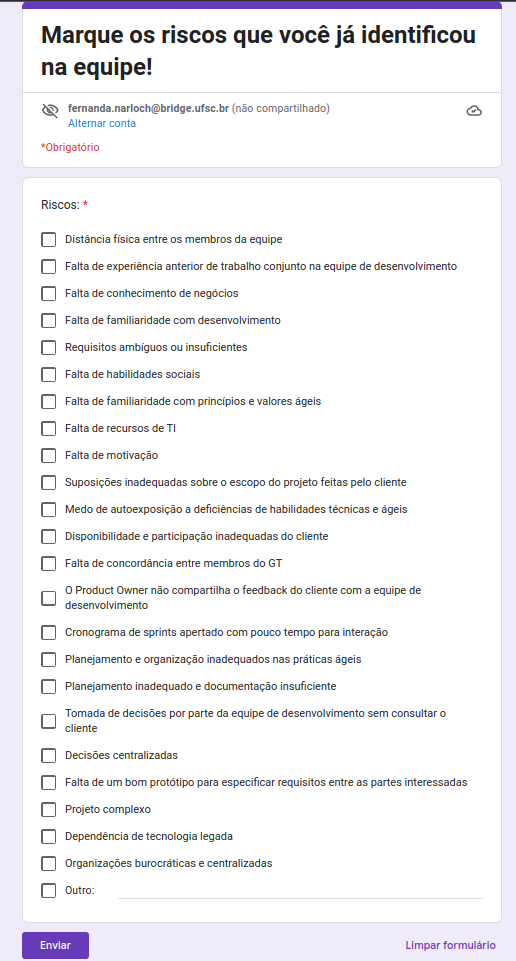
\includegraphics[width=0.8\textwidth]{src/tex/img/modelo-formulario.png}
    \caption{Modelo de formulário para identificação de riscos}
    \label{fig:form_model}
\end{figure}

Depois de identificados, os riscos são automaticamente alocados em uma linha da planilha e podem, então, ser posteriormente analisados de acordo com a técnica selecionada pela equipe. Além da descrição do risco, a planilha também permite que os membros das equipes avaliem o risco em Impacto ("Insignificante", "Moderado" e "Catastrófico") e em Probabilidade ("Baixa", "Média" e "Alta"). Na Figura \ref{fig:checklist_ex} é apresentado o modelo de planilha utilizado pelas equipes. Também foi disponibilizada a Matriz de Riscos abaixo para que as equipes possam definir a prioridade do risco. 

\begin{table}[H]
\centering
\caption{Matriz de riscos utilizada}
\begin{tabular}{|l|l|l|l|}
\rowcolor[HTML]{FFFFFF} 
\multicolumn{4}{c}{\cellcolor[HTML]{FFFFFF}{\color[HTML]{333333} \textbf{Prioridade}}}                                                                                     \\\hline
\rowcolor[HTML]{FFCCC9} 
\cellcolor[HTML]{C0C0C0}{\color[HTML]{333333} \textbf{Alta}}  & \cellcolor[HTML]{FFFC9E}Média         & Alta                            & Alta                                \\\hline
\cellcolor[HTML]{C0C0C0}{\color[HTML]{333333} \textbf{Média}} & \cellcolor[HTML]{9AFF99}Baixa         & \cellcolor[HTML]{FFFC9E}Média   & \cellcolor[HTML]{FFCCC9}Alta        \\\hline
\rowcolor[HTML]{9AFF99} 
\cellcolor[HTML]{C0C0C0}{\color[HTML]{333333} \textbf{Baixa}} & Baixa                                 & Baixa                           & \cellcolor[HTML]{FFFC9E}Média       \\\hline
\rowcolor[HTML]{C0C0C0} 
{\color[HTML]{333333} \textbf{Probabilidade/Impacto}}         & {\color[HTML]{333333} \textbf{Insignificante}} & {\color[HTML]{333333} \textbf{Moderado}} & {\color[HTML]{333333} \textbf{Catastrófico}} \\\hline
\end{tabular}
\\
{\textbf{Fonte:} Desenvolvido pela autora (2022)}
\end{table}

\begin{figure}
    \centering
    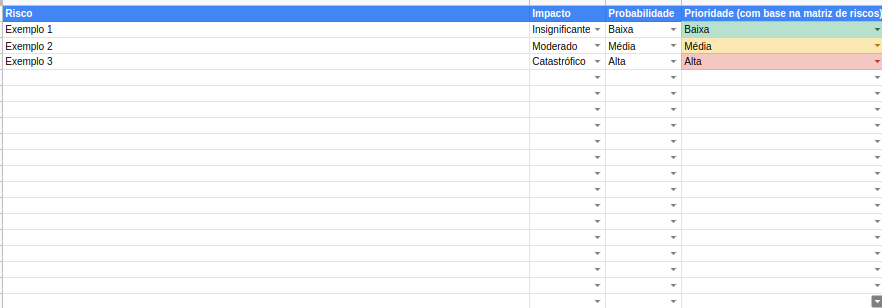
\includegraphics[width=1\textwidth]{src/tex/img/checklist-exemplo.png}
    \caption{Modelo de planilha utilizada para a Checklist de Riscos}
    \label{fig:checklist_ex}
\end{figure}

Ambas as equipes optaram por realizar a análise dos riscos durante a cerimônia de Daily Scrum, ao final de cada \textit{sprint}. Já a identificação dos riscos ocorreu de forma recorrente.

Além das ferramentas descritas, também foi utilizado um cronômetro digital para medir o tempo gasto na aplicação das técnicas durante a cerimônia de Daily Scrum e as planilhas de acompanhamento próprias das equipes de onde serão analisadas o esforço estimado e real da equipe durante a aplicação das abordagens. 

\section{Aplicação dos métodos de gestão de risco nas equipes}

A aplicação do estudo de caso ocorreu em três \textit{sprints} distintas entre os meses de Setembro e Novembro de 2022.

O início das aplicações dos métodos ocorreu no dia 26 de Setembro de 2022 em ambas as equipes. Isso se deu através da divulgação para as equipes das ferramentas de identificação e análise e também de um vídeo com uma breve explicação sobre o uso das ferramentas. No vídeo, foram apresentadas as técnicas de gestão de risco selecionadas, o formulário para preenchimento pelos membros da equipe e também a planilha para qual os riscos foram mapeados.

Assim, durante as próximas três \textit{sprints} de duas semanas cada, os participantes ficaram livres para aplicar as técnicas da forma que considerassem mais adequada para o contexto da equipe. 

\subsection{Aplicação na equipe F}

Em primeiro lugar, o vídeo explicativo foi disponibilizado no canal da equipe da ferramenta Slack no dia 26 de Setembro de 2022. Em conjunto ao vídeo, também foram disponibilizadas as ferramentas para identificação e análise dos riscos. 

O formulário da equipe F recebeu 6 respostas durante a primeira \textit{sprint} de aplicação da técnica de identificação de riscos e, segundo os participantes, cada membro respondeu ao formulário uma única vez. 

Os riscos identificados pela equipe foram majoritariamente os já presentes na lista de apoio. Com maior aparição dos riscos "Projeto complexo" e "Dependência de tecnologias legadas". Na Figura \ref{fig:result_found} é apresentada a relação de cada risco identificado e a porcentagem de respostas que o incluíram.

\begin{figure}[H]
    \centering
    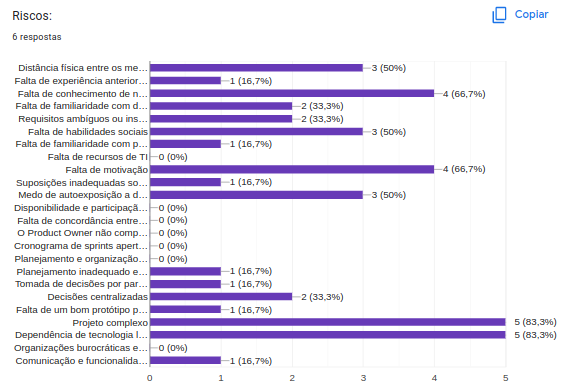
\includegraphics[width=0.8\textwidth]{src/tex/img/resultado-foundation.png}
    \caption{Resultado da identificação de riscos da equipe F}
    \label{fig:result_found}
\end{figure}

Após a identificação dos riscos, na \textit{sprint} seguinte, os participantes realizaram a análise dos riscos através da aplicação da Matriz de Riscos. Esse processo foi realizado de forma síncrona no dia 17 de Outubro de 2022 durante uma reunião por videoconferência após a cerimônia de Daily Scrum. 

A discussão teve início às 15h58 e estendeu-se por 53 minutos até 16h51. Durante esse processo, a equipe avaliou cada um dos riscos identificados e atribuiu um valor para o Impacto e outro para a Probabilidade para, então, calcular a Prioridade a partir da Matriz de Riscos. O resultado da priorização está compilado na Figura \ref{fig:result_found}.

\begin{figure}[H]
    \centering
    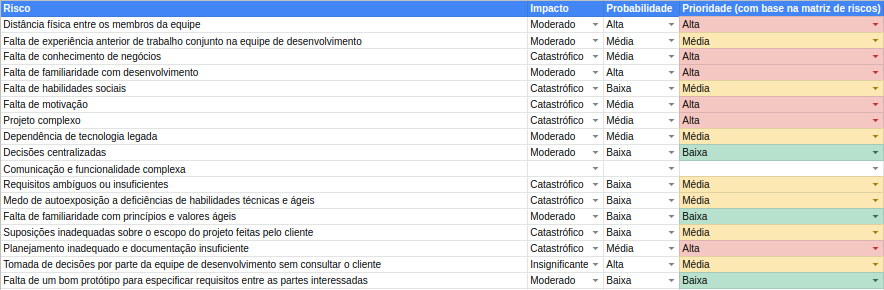
\includegraphics[width=1\textwidth]{src/tex/img/riscos_founds.png}
    \caption{Resultado da análise de riscos da equipe F}
    \label{fig:result_found}
\end{figure}

A equipe F obteve 6 riscos de alta prioridade, 7 de média e 3 de baixa. Além disso, um risco que foi preenchido através do campo "Outro" no formulário não foi compreendido pela equipe e, sendo assim, não foi avaliado.

\subsection{Aplicação na equipe FN}

A equipe FN também teve os vídeos explicativos e ferramentas divulgados no mesmo dia da equipe F. Porém, em um primeiro momento a equipe apresentou dificuldades na identificação de riscos. As primeiras respostas foram obtidas apenas durante a segunda \textit{sprint} da aplicação e apenas uma identificou um risco no projeto: "Organizações burocráticas e centralizadas". Em duas outras respostas os membros relataram não terem identificado riscos.

Contudo, durante a terceira \textit{sprint}, foram obtidas novas respostas ao formulário que englobavam tanto riscos presentes na Checklist quanto riscos identificados individualmente pelos participantes. O risco de maior destaque foi a imprevisibilidade por parte do cliente.

A relação dos riscos identificados pela equipe se encontra na figura abaixo:

\begin{figure}[H]
    \centering
    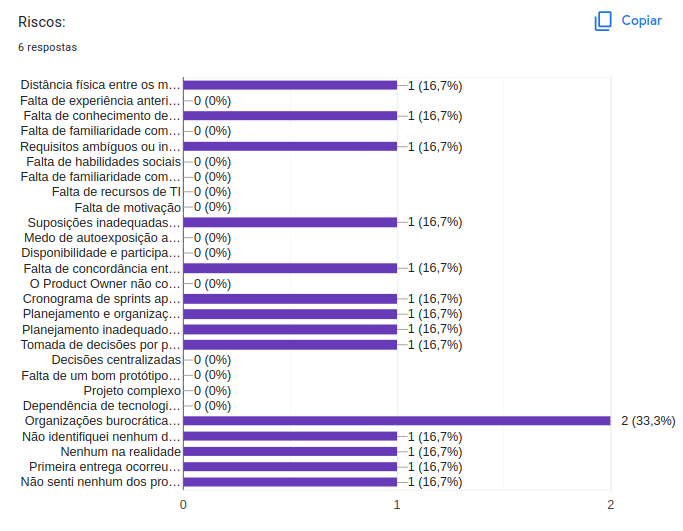
\includegraphics[width=0.8\textwidth]{src/tex/img/riscos-fruit.png}
    \caption{Resultado da identificação de riscos da equipe FN}
    \label{fig:risk_fruit}
\end{figure}

Alguns riscos obtidos precisaram ser ajustados para a planilha, pois continham mais de um risco descrito no campo de texto livre. Após esse ajuste, a equipe realizou durante a primeira semana de Novembro a priorização dos riscos utilizando a Matriz de Riscos. A priorização também foi realizada de forma assíncrona, no caso desta equipe o \textit{Product Owner} coletou individualmente as opiniões sobre cada um dos riscos através do Slack e preencheu depois preencheu a tabela com os resultados. Apresentando-os porteriormente para a equipe. O resultado da aplicação encontra-se na Figura \ref{fig:result_fruit}.

\begin{figure}[H]
    \centering
    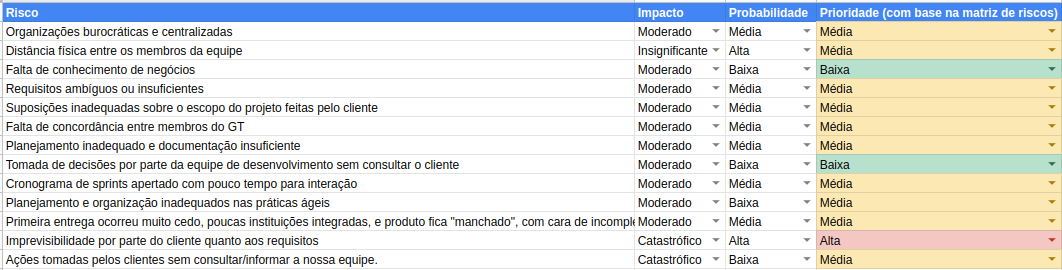
\includegraphics[width=1\textwidth]{src/tex/img/resultado-fruit.png}
    \caption{Resultado da análise de riscos da equipe FN}
    \label{fig:result_fruit}
\end{figure}

\subsection{Coleta de dados}

O período de coleta de dados iniciou-se em conjunto com a aplicação do estudo de caso, no dia 26 de Setembro de 2022, e foi encerrado no dia 18 de Novembro de 2022. Primeiramente, não foi realizada uma intervenção para a coleta de dados e foram apenas reunidas as estimativas de esforço de cada equipe. Os artefatos gerados pelas duas equipes durante a aplicação também foram coletados e podem ser encontrados no Apêndice \ref{sec:ApendiceC}. 
Já para a coleta de medidas referentes aos objetivos 2 e 3 das medições, foi aplicado um questionário (vide Apêndice \ref{sec:ApendiceB}) ao final da terceira \textit{sprint}, entre os dias 7 e 18 de Novembro. O questionário foi enviado a todos os membros das equipes participantes. Já a medida relacionada ao tempo gasto para a aplicação das técnicas foi obtido através de um cronômetro digital utilizado durante as cerimônias para priorização dos riscos. Contudo, apenas a equipe "F" fez uso dessa ferramenta, pois a equipe "FN" realizou esta etapa de maneira assíncrona.

\section{Análise dos dados}

\begin{table}[H]
\begin{tabular}{|
>{\columncolor[HTML]{C0C0C0}}l |l|}
\hline
\multicolumn{1}{|c|}{\cellcolor[HTML]{C0C0C0}{\color[HTML]{333333} \textbf{Pergunta 1.1}}} &  \begin{tabular}[c]{@{}l@{}}Qual o esforço total despendido pelas áreas de análise, desen-\\ volvimento e teste para aplicação de técnicas de gestão de risco?\end{tabular}
 \\ \hline
{\color[HTML]{333333} \textbf{Medição 1.1}}                                                & Esforço total em horas pelo número de participantes. \\ \hline
\end{tabular}
\end{table}

\begin{table}[H]
\begin{tabular}{|
>{\columncolor[HTML]{C0C0C0}}l |l|}
\hline
\multicolumn{1}{|c|}{\cellcolor[HTML]{C0C0C0}{\color[HTML]{333333} \textbf{Pergunta 2.1}}} &  \begin{tabular}[c]{@{}l@{}}As técnicas de gestão de risco são de fácil compreensão e aplica-\\ção?\end{tabular}
 \\ \hline
{\color[HTML]{333333} \textbf{Medição 2.1}}                                                & \begin{tabular}[c]{@{}l@{}}Impressão subjetiva das principais técnicas de gestão de risco apli-\\cadas.\end{tabular} \\ \hline
\end{tabular}
\end{table}

Como você classificaria a facilidade de compreensão e utilização das técnicas de gestão de risco apresentadas? Por quê?

\begin{table}[H]
\begin{tabular}{|
>{\columncolor[HTML]{C0C0C0}}l |l|}
\hline
\multicolumn{1}{|c|}{\cellcolor[HTML]{C0C0C0}{\color[HTML]{333333} \textbf{Pergunta 2.2}}} &  \begin{tabular}[c]{@{}l@{}}A experiência da aplicação da abordagem foi benéfica a equipe?\end{tabular}
 \\ \hline
{\color[HTML]{333333} \textbf{Medição 2.2}}                                                & \begin{tabular}[c]{@{}l@{}}Impressão subjetiva das principais técnicas de gestão de risco apli-\\cadas.\end{tabular} \\ \hline
\end{tabular}
\end{table}

Quão benéfica foi para a equipe a aplicação das técnicas? Por quê?\\

\begin{table}[H]
\begin{tabular}{|
>{\columncolor[HTML]{C0C0C0}}l |l|}
\hline
\multicolumn{1}{|c|}{\cellcolor[HTML]{C0C0C0}{\color[HTML]{333333} \textbf{Pergunta 2.3}}} &  \begin{tabular}[c]{@{}l@{}}Quais foram as principais dificuldades encontradas na aplicação \\das técnicas de gestão de risco?\end{tabular}
 \\ \hline
{\color[HTML]{333333} \textbf{Medição 2.3}}                                                & \begin{tabular}[c]{@{}l@{}}Impressão subjetiva das principais técnicas de gestão de risco apli-\\cadas.\end{tabular} \\ \hline
\end{tabular}
\end{table}

Quais foram as principais dificuldades encontradas na aplicação das técnicas? \\ \\

\begin{table}[H]
\begin{tabular}{|
>{\columncolor[HTML]{C0C0C0}}l |l|}
\hline
\multicolumn{1}{|c|}{\cellcolor[HTML]{C0C0C0}{\color[HTML]{333333} \textbf{Pergunta 2.4}}} &  \begin{tabular}[c]{@{}l@{}} Houve impacto na velocidade da equipe ao aplicar técnicas de \\gestão de risco?\end{tabular}
 \\ \hline
{\color[HTML]{333333} \textbf{Medição 2.4}}                                                & \begin{tabular}[c]{@{}l@{}}Diferença percentual entre a estimativa de esforço da equipe ao \\aplicar técnicas de gestão de risco em relação a estimativa de
esforço \\da mesma equipe antes da aplicação da abordagem.\end{tabular} \\ \hline
\end{tabular}
\end{table}

\begin{table}[H]
\begin{tabular}{|
>{\columncolor[HTML]{C0C0C0}}l |l|}
\hline
\multicolumn{1}{|c|}{\cellcolor[HTML]{C0C0C0}{\color[HTML]{333333} \textbf{Pergunta 3.1}}} &  \begin{tabular}[c]{@{}l@{}} A equipe pretende continuar utilizando as técnicas apresentadas? Se\\ sim, porquê?\end{tabular}
 \\ \hline
{\color[HTML]{333333} \textbf{Medição 3.1}}                                                & \begin{tabular}[c]{@{}l@{}}Impressão subjetiva das principais técnicas de gestão de risco apli-\\cadas.\end{tabular} \\ \hline
\end{tabular}
\end{table}

Você continuaria utilizando uma das técnicas apresentadas? Por quê? \\ 

\begin{table}[H]
\begin{tabular}{|
>{\columncolor[HTML]{C0C0C0}}l |l|}
\hline
\multicolumn{1}{|c|}{\cellcolor[HTML]{C0C0C0}{\color[HTML]{333333} \textbf{Pergunta 2.4}}} &  \begin{tabular}[c]{@{}l@{}} Quais foram os principais pontos positivos, sob o ponto de vista das \\áreas de análise, desenvolvimento e teste, na aplicação das técnicas\\ para gestão de risco?\end{tabular}
 \\ \hline
{\color[HTML]{333333} \textbf{Medição 2.4}}                                                & \begin{tabular}[c]{@{}l@{}}Impressão subjetiva das principais técnicas de gestão de risco apli-\\cadas.\end{tabular} \\ \hline
\end{tabular}
\end{table}

    Quais foram os principais pontos positivos resultantes da aplicação das técnicas para gestão de riscos? \\ \\


\section{Discussão}

  \postextual


  % ----------------------------------------------------------
  % Referências bibliográficas
  % ----------------------------------------------------------
  \bibliography{references}
  
  % ----------------------------------------------------------
  % Glossário
  % ----------------------------------------------------------
  %
  % Consulte o manual da classe abntex2 para orientações sobre o glossário.
  %
  %\glossary
  


  % ----------------------------------------------------------
  % Apêndices
  % ----------------------------------------------------------

  % ---
  % Inicia os apêndices
  % ---
  \begin{apendicesenv}
    
  % Imprime uma página indicando o início dos apêndices
  \partapendices
  % ----------------------------------------------------------
 \chapter{Estudos Selecionados no Mapeamento Sistemático da Literatura}
 \label{sec:ApendiceA}
 
 O quadro abaixo apresenta os estudos selecionados durante a Mapeamento Sistemático da Literatura.

\begin{longtable}{|p{1cm}|p{4cm}|p{10cm}|}
    \centering
            \rowcolor{lightgray}
            \textbf{ID} & \textbf{Título} & \textbf{Referência} 
            \\ \hline 

            \flushleft{\textbf{[1]}} & \flushleft{\textit{Reference framework and model for integration of risk management in agile systems engineering lifecycle of the defense acquisition management framework}} & \flushleft{CROWE, Portia; MOSTASHARI, Ali; MANSOURI, Mo; CLOUTIER, Robert. 9.2.1 Reference Framework and Model for Integration of Risk Management in Agile Systems Engineering Lifecycle of the Defense Acquisition Management Framework. \textbf{Incose International Symposium}, [S.L.], v. 19, n. 1, p. 1391-1405, jul. 2009. Wiley. http://dx.doi.org/10.1002/j.2334-5837.2009.tb01022.x.}
            \\ \hline

            \flushleft{\textbf{[2]}} & \flushleft{\textit{A risk management framework for distributed scrum using prince2 methodology}} & \flushleft{ESTEKI, Mohammad; GANDOMANI, Taghi Javdani; FARSANI, Hadi Khosravi. A risk management framework for distributed scrum using PRINCE2 methodology. \textbf{Bulletin Of Electrical Engineering And Informatics}, [S.L.], v. 9, n. 3, p. 1299-1310, 1 jun. 2020. Institute of Advanced Engineering and Science. http://dx.doi.org/10.11591/eei.v9i3.1905.}
            \\ \hline 
            
            \flushleft{\textbf{[3]}} & \flushleft{\textit{A Risk Management Tool for Agile Software Development}} & \flushleft{TAVARES, Breno Gontijo; KEIL, Mark; SILVA, Carlos Eduardo Sanches da; SOUZA, Adler Diniz de. A Risk Management Tool for Agile Software Development. \textbf{Journal Of Computer Information Systems}, [S.L.], p. 1-10, 7 dez. 2020. Informa UK Limited. http://dx.doi.org/10.1080/08874417.2020.1839813.}
            \\ \hline \hline
            
            \flushleft{\textbf{[4]}} & \flushleft{\textit{Improving Risk Management in a Scaled Agile Environment}} & \flushleft{SCHÖN, Eva-Maria; RADTKE, Dirk; JORDAN, Christian. Improving Risk Management in a Scaled Agile Environment. \textbf{Lecture Notes In Business Information Processing}, [S.L.], p. 132-141, 2020. Springer International Publishing. http://dx.doi.org/10.1007/978-3-030-49392-99}
            \\ \hline        
 
            \flushleft{\textbf{[5]}} & \flushleft{\textit{Risk assessment forum: A proposal for agile software development teams ruled by Scrum}} & \flushleft{CARVALLO, Juliette Michelle Parada; OKTABA, Hanna; HERNANDEZ, Elsa Ramirez. Risk Assessment Forum. \textbf{2018 6Th International Conference In Software Engineering Research And Innovation (Conisoft)}, [S.L.], p. 132-141, out. 2018. IEEE. http://dx.doi.org/10.1109/conisoft.2018.8645949.}
            \\ \hline
            
            \flushleft{\textbf{[6]}} & \flushleft{\textit{Agile risk management using software agents}} & \flushleft{ODZALY, Edzreena Edza; GREER, Des; STEWART, Darryl. Agile risk management using software agents. \textbf{Journal Of Ambient Intelligence And Humanized Computing}, [S.L.], v. 9, n. 3, p. 823-841, 2 maio 2017. Springer Science and Business Media LLC. http://dx.doi.org/10.1007/s12652-017-0488-2.}
            \\ \hline               

            \flushleft{\textbf{[7]}} & \flushleft{\textit{A risk poker based testing model for scrum}} & \flushleft{GHAZALI, Siti Noor Hasanah; SALIM, Siti Salwah; INAYAT, Irum; HAMID, Siti Hafizah Ab. A Risk Poker Based Testing Model for Scrum. \textbf{Computer Systems Science And Engineering}, [S.L.], v. 33, n. 3, p. 169-185, 2018. Computers, Materials and Continua (Tech Science Press). http://dx.doi.org/10.32604/csse.2018.33.169.} 
            \\ \hline \hline  
            
            \flushleft{\textbf{[8]}} & \flushleft{\textit{Agile approach with Kanban in information security risk management}} & \flushleft{DORCA, Vasile; MUNTEANU, Radu; POPESCU, Sorin; CHIOREANU, Adrian; PELESKEI, Claudius. Agile approach with Kanban in information security risk management. \textbf{2016 Ieee International Conference On Automation, Quality And Testing, Robotics (Aqtr)}, [S.L.], p. 1-6, maio 2016. IEEE. http://dx.doi.org/10.1109/aqtr.2016.7501278.}
            \\ \hline                
 
            \flushleft{\textbf{[9]}} & \flushleft{\textit{Integrating Risk Management in Scrum Framework}} & \flushleft{HAMMAD, Muhammad; INAYAT, Irum. Integrating Risk Management in Scrum Framework.\textbf{ 2018 International Conference On Frontiers Of Information Technology (Fit)}, [S.L.], p. 158-163, dez. 2018. IEEE. http://dx.doi.org/10.1109/fit.2018.00035.}
            \\ \hline         
            
            \flushleft{\textbf{[10]}} & \flushleft{\textit{Prioritizing and optimizing risk factors in agile software development}} & \flushleft{ AGRAWAL, Ruchi; SINGH, Deepali; SHARMA, Ashish. Prioritizing and optimizing risk factors in agile software development. \textbf{2016 Ninth International Conference On Contemporary Computing (Ic3)}, [S.L.], p. 1-7, ago. 2016. IEEE. http://dx.doi.org/10.1109/ic3.2016.7880232.}
            \\ \hline
 
            \flushleft{\textbf{[11]}} & \flushleft{\textit{Value-Risk Trade-off Analysis for Iteration Planning in Extreme Programming}} & \flushleft{DONG, Xin; YANG, Qiu-Song; WANG, Qing; ZHAI, Jian; RUHE, Gunther. Value-Risk Trade-off Analysis for Iteration Planning in Extreme Programming. \textbf{2011 18Th Asia-Pacific Software Engineering Conference}, [S.L.], p. 397-404, dez. 2011. IEEE. http://dx.doi.org/10.1109/apsec.2011.11.}
            \\ \hline \hline
            
            \flushleft{\textbf{[12]}} & \flushleft{\textit{A case study for the implementation of an agile risk management process in multiple projects environments}} & \flushleft{RIBEIRO, Lucio; GUSMAO, Cristine; FEIJO, Wilmar; BEZERRA, Vicente. A case study for the implementation of an agile risk management process in multiple projects environments. \textbf{Picmet '09 - 2009 Portland International Conference On Management Of Engineering \& Technology}, [S.L.], p. 1396-1404, ago. 2009. IEEE. http://dx.doi.org/10.1109/picmet.2009.5262002.}
            \\ \hline                

            \flushleft{\textbf{[13]}} & \flushleft{\textit{A SYSML-Based Approach for Requirements Risk Management and Change Control}} & \flushleft{HAYAT, Faisal; ANWAR, Muhammad Waseem; AZAM, Farooque; KIRAN, Ayesha. A SYSML-Based Approach for Requirements Risk Management and Change Control. Proceedings Of The 2019 11Th International Conference On Information Management And Engineering, [S.L.], p. 20-24, 19 set. 2019. ACM. http://dx.doi.org/10.1145/3373744.3373751.}
            \\ \hline \hline   
            
            \flushleft{\textbf{[14]}} & \flushleft{\textit{Risk Management for Agile Projects in Offshore Vietnam}} & \flushleft{CUONG, Le Gia; HUNG, Phan Duy; BACH, Nguyen Luu; TUNG, Ta Duc. Risk Management for Agile Projects in Offshore Vietnam. \textbf{Proceedings Of The Tenth International Symposium On Information And Communication Technology - Soict 2019}, [S.L.], p. 377-384, 2019. ACM Press. http://dx.doi.org/10.1145/3368926.3369718.}
            \\ \hline \hline   
            
            \flushleft{\textbf{[15]}} & \flushleft{\textit{An industrial case study of implementing software risk management}} & \flushleft{FREIMUT, Bernd; HARTKOPF, Susanne; KAISER, Peter; KONTIO, Jyrki; KOBITZSCH, Werner. An industrial case study of implementing software risk management. \textbf{Acm Sigsoft Software Engineering Notes}, [S.L.], v. 26, n. 5, p. 277-287, set. 2001. Association for Computing Machinery (ACM). http://dx.doi.org/10.1145/503271.503247.}
            \\ \hline    
            
            \flushleft{\textbf{[16]}} & \flushleft{\textit{Characterization of risky projects based on project managers' evaluation}} & \flushleft{MIZUNO, Osamu; KIKUNO, Tohru; TAKAGI, Yasunari; SAKAMOTO, Keishi. 22ND INTERNATIONAL CONFERENCE ON SOFTWARE ENGINEERING (ICSE '00), 2000, Limerick. \textbf{Characterization of risky projects based on project managers' evaluation.} Nova Iorque: Association For Computing Machinery, 2000.}
            \\ \hline   
            
            \flushleft{\textbf{[17]}} & \flushleft{\textit{Characterization and prediction of issue-related risks in software projects}} & \flushleft{CHOETKIERTIKUL, Morakot; DAM, Hoa Khanh; TRAN, Truyen; GHOSE, Aditya. Characterization and Prediction of Issue-Related Risks in Software Projects. \textbf{2015 Ieee/Acm 12Th Working Conference On Mining Software Repositories}, [S.L.], maio 2015. IEEE. http://dx.doi.org/10.1109/msr.2015.33.}
            \\ \hline 
            
            \addlinespace[0.2cm]
            \caption*{\textbf{Fonte:} Desenvolvido pela autora (2021).}
\end{longtable}

 \chapter{Questionário a ser aplicado nas equipes do estudo}
 \label{sec:ApendiceB}
 
 Este questionário foi desenvolvido pela acadêmica Fernanda Narloch Rizzo Hahn, aluna
do curso de Ciências da Computação da Universidade Federal de Santa Catarina, como
parte de seu Trabalho de Conclusão de Curso. Tem como proposta implantar e avaliar técnicas de gestão de risco no contexto ágil de uma unidade organizacional, por meio de um estudo de caso aplicado nas equipes ágeis do Laboratório Bridge da Universidade Federal de Santa Catarina.

\textbf{Cargo:}\hspace*{250pt}\textbf{Data:}

\begin{itemize} [label={}]
    \item \textbf{1 - } Como você classificaria a facilidade de compreensão e utilização das técnicas de gestão de risco apresentadas? Por quê? \\ \\
    \item \textbf{2 - } Você continuaria utilizando uma das técnicas apresentadas? Por quê? \\ \\
    \item \textbf{3 - } Quão benéfica foi para a equipe a aplicação das técnicas? Por quê? \\ \\
    \item \textbf{4 - } Quais foram as principais dificuldades encontradas na aplicação das técnicas? \\ \\
    \item \textbf{5 - } Quais foram os principais pontos positivos resultantes da aplicação das técnicas para gestão de riscos? \\ \\
    \item \textbf{6 - } Você tem alguma sugestão? \\ \\

\end{itemize}

 \chapter{Artefatos gerados pelas equipes}
 \label{sec:ApendiceC}
 \section{Equipe F}
\subsection{Dados brutos planilha}

\begin{figure}[H]
    \centering
    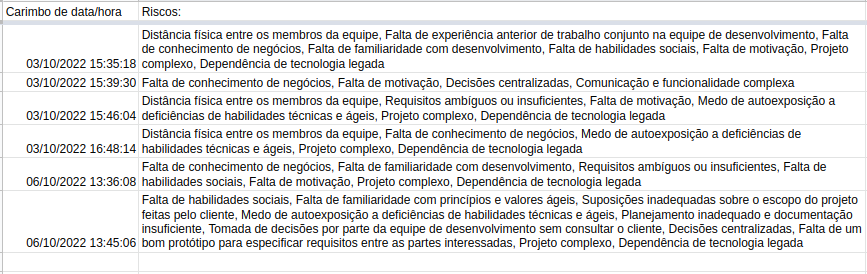
\includegraphics[width=1\textwidth]{src/tex/img/dados-founds.png}
\end{figure}

\subsection{Resultado da Checklist}

\begin{figure}[H]
    \centering
    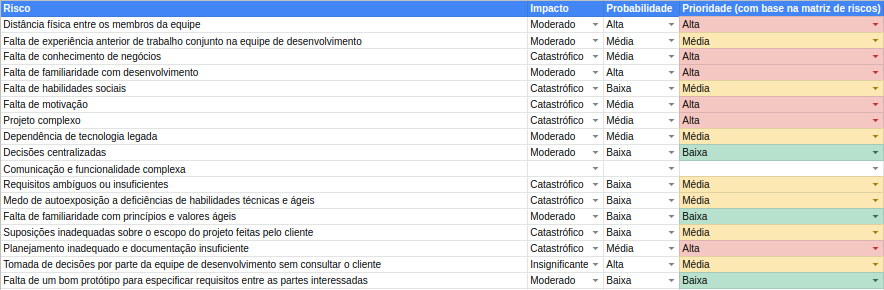
\includegraphics[width=1\textwidth]{src/tex/img/riscos_founds.png}
\end{figure}

\subsection{Respostas do formulário}
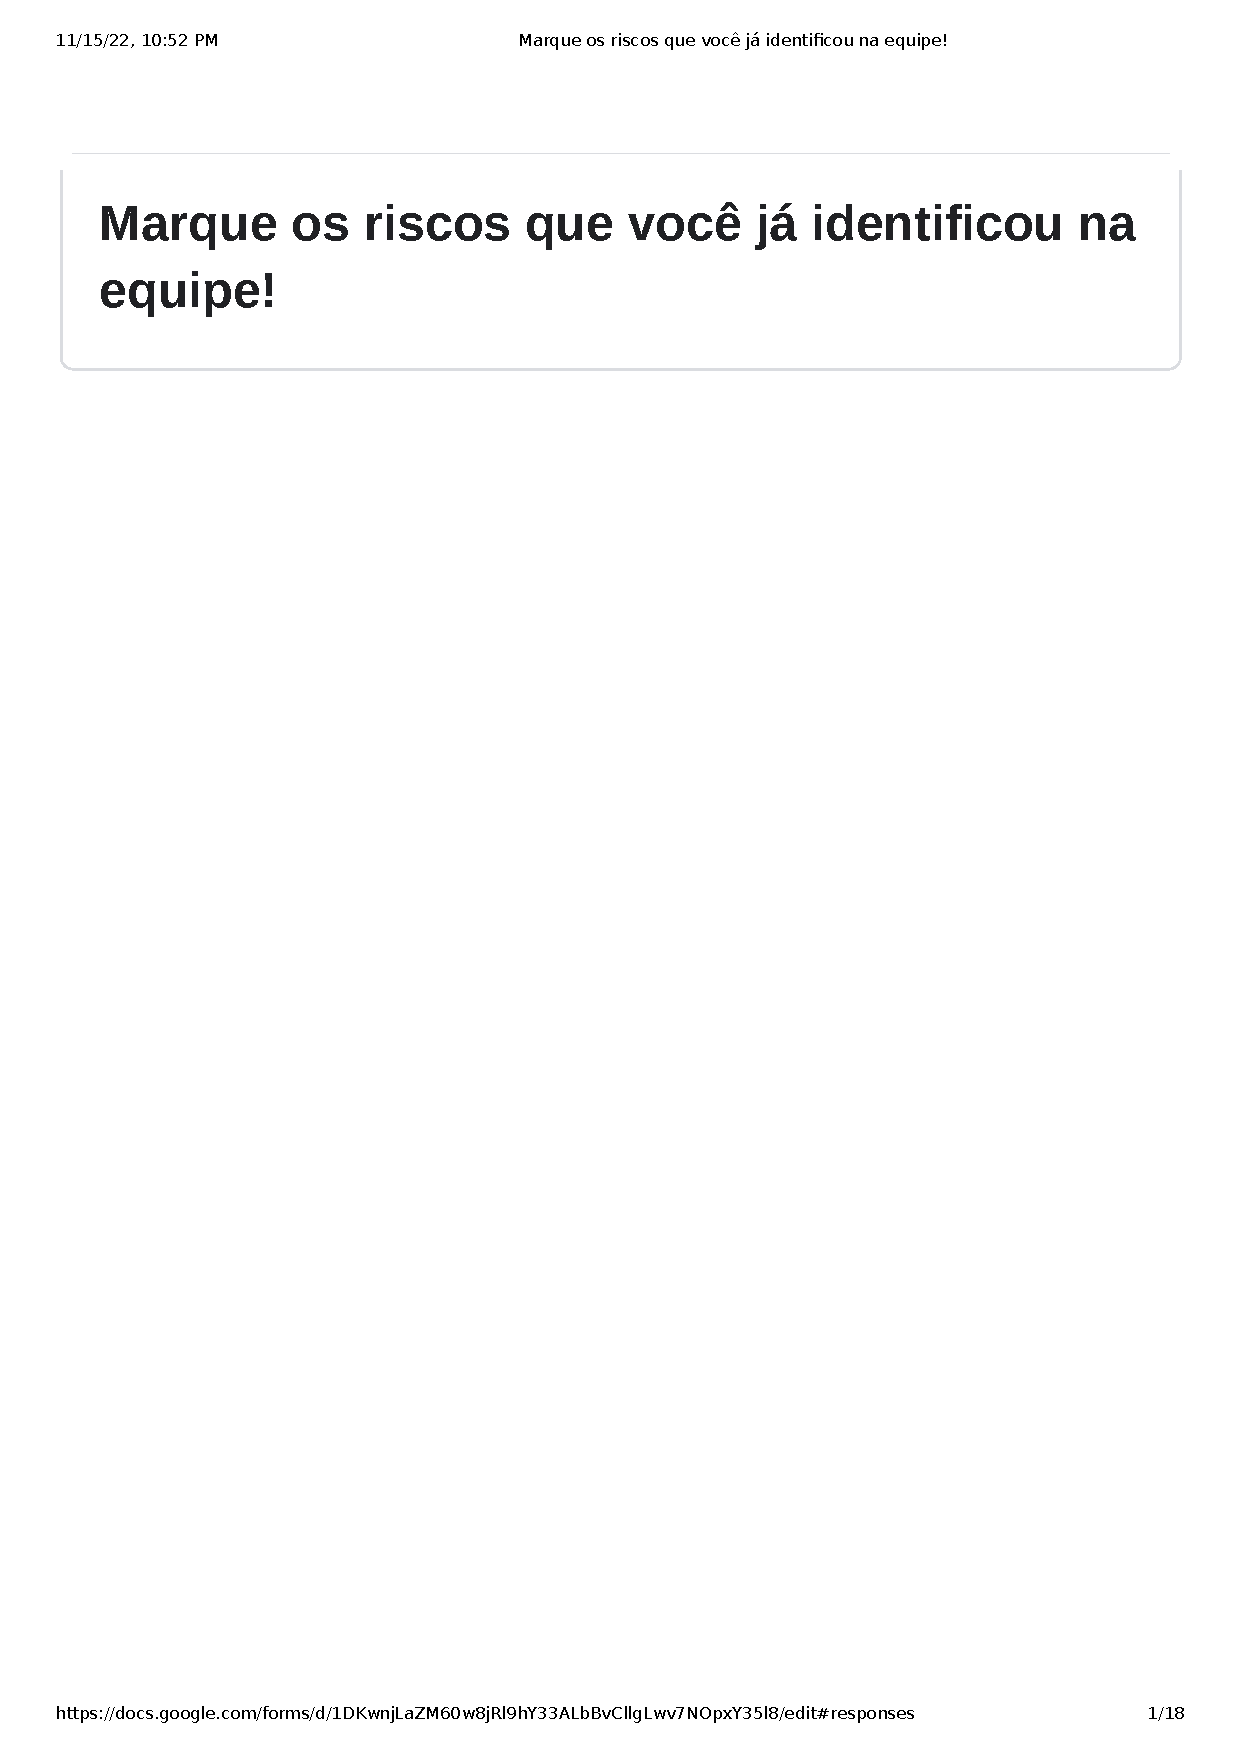
\includepdf[pages=-]{form-founds.pdf}
 
 
\section{Equipe FN}
\subsection{Dados brutos planilha}

\begin{figure}[H]
    \centering
    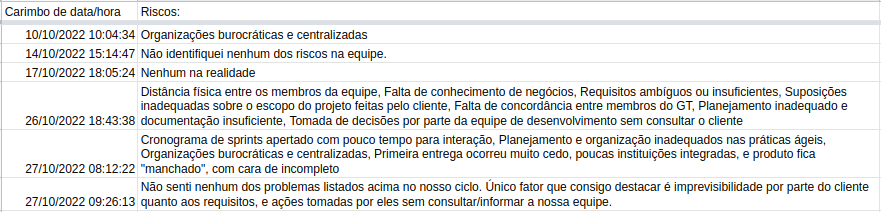
\includegraphics[width=1\textwidth]{src/tex/img/dados-fn.png}
\end{figure}

\subsection{Resultado da Checklist}

\begin{figure}[H]
    \centering
    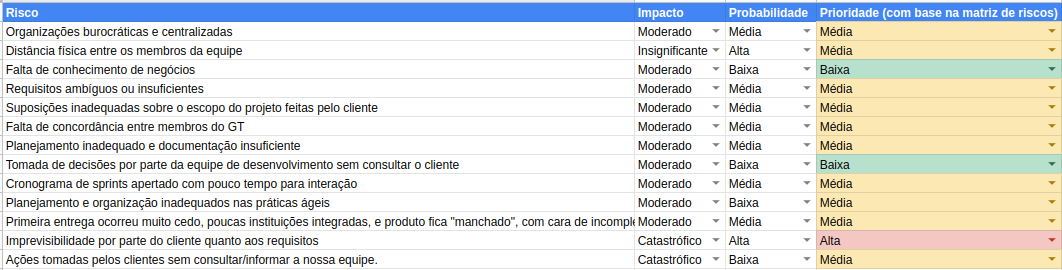
\includegraphics[width=1\textwidth]{src/tex/img/resultado-fruit.png}
\end{figure}

\subsection{Respostas do formulário}
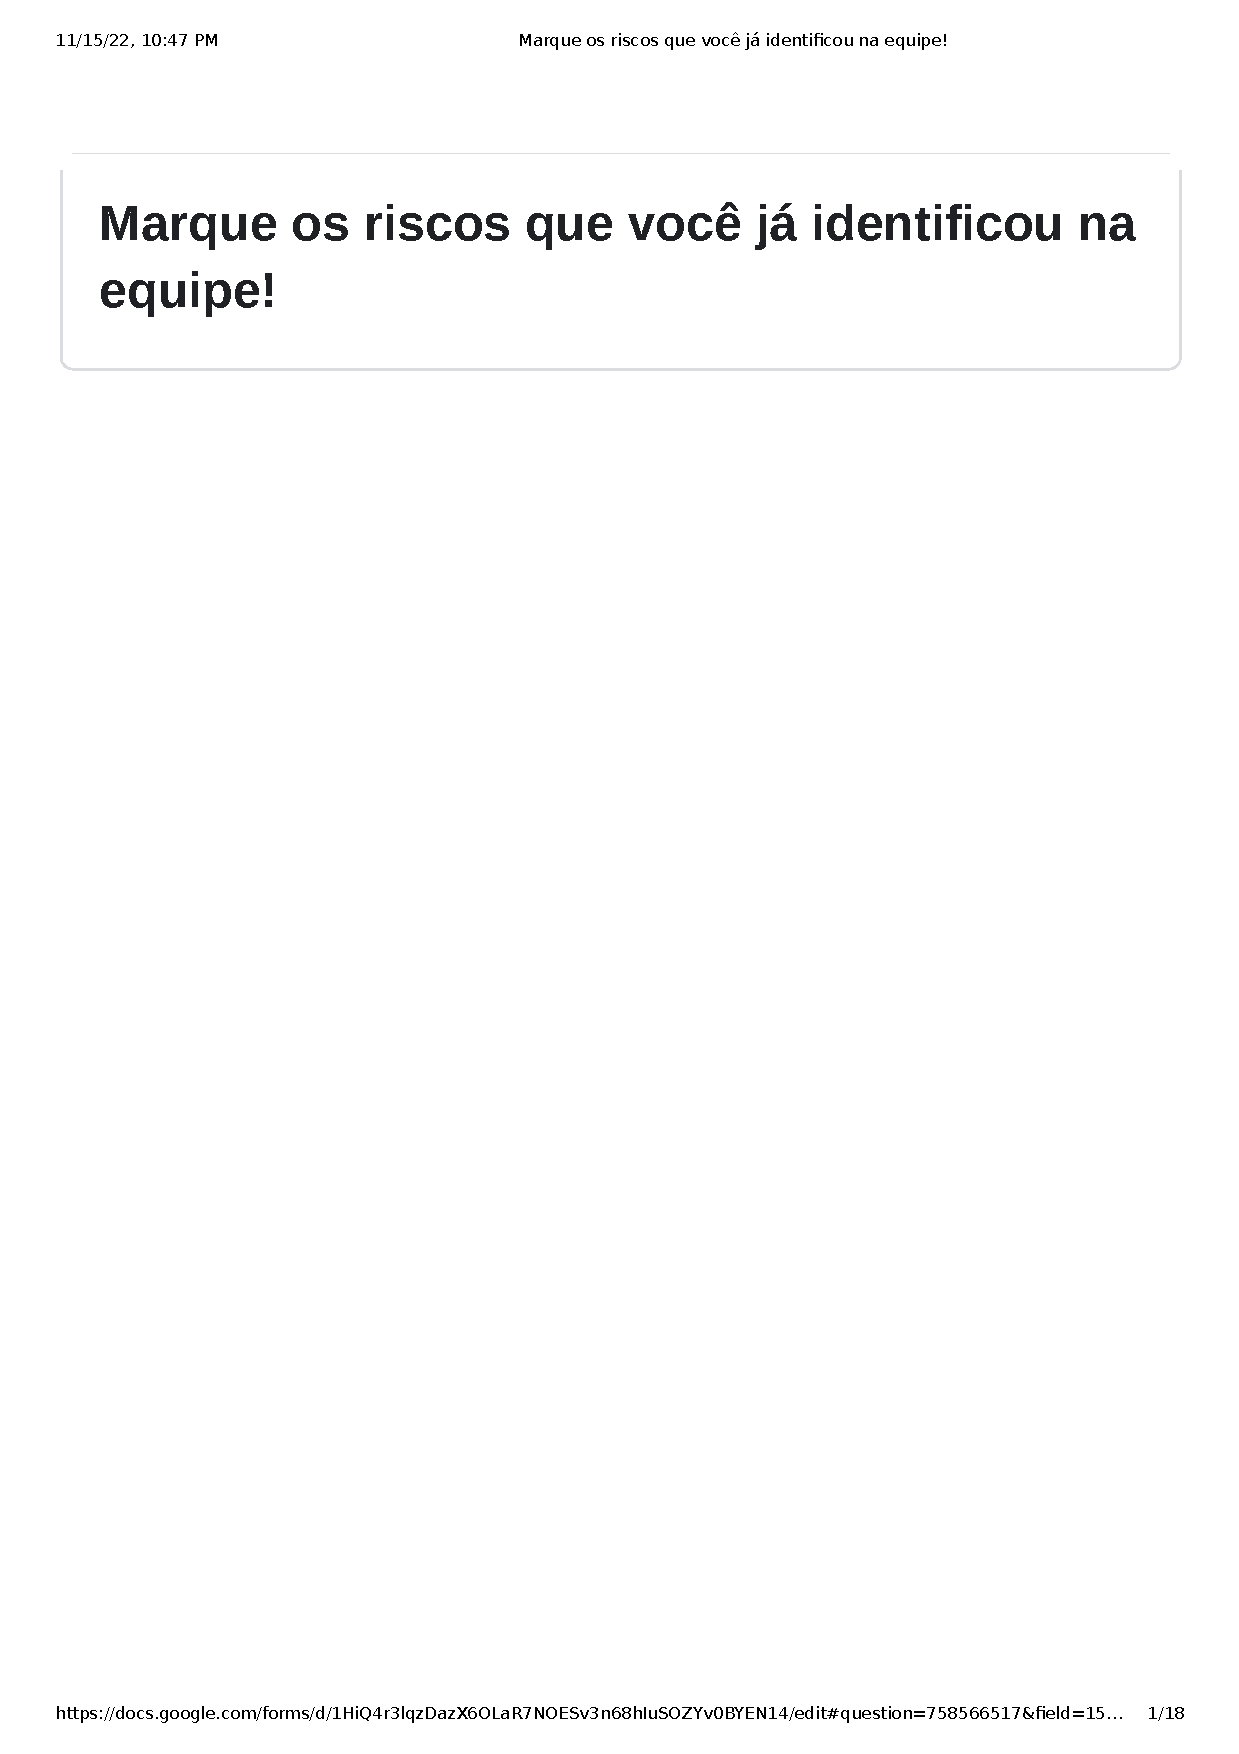
\includepdf[pages=-]{form-fn.pdf}

 \chapter{Artigo desenvolvido}
 \label{sec:ApendiceD}
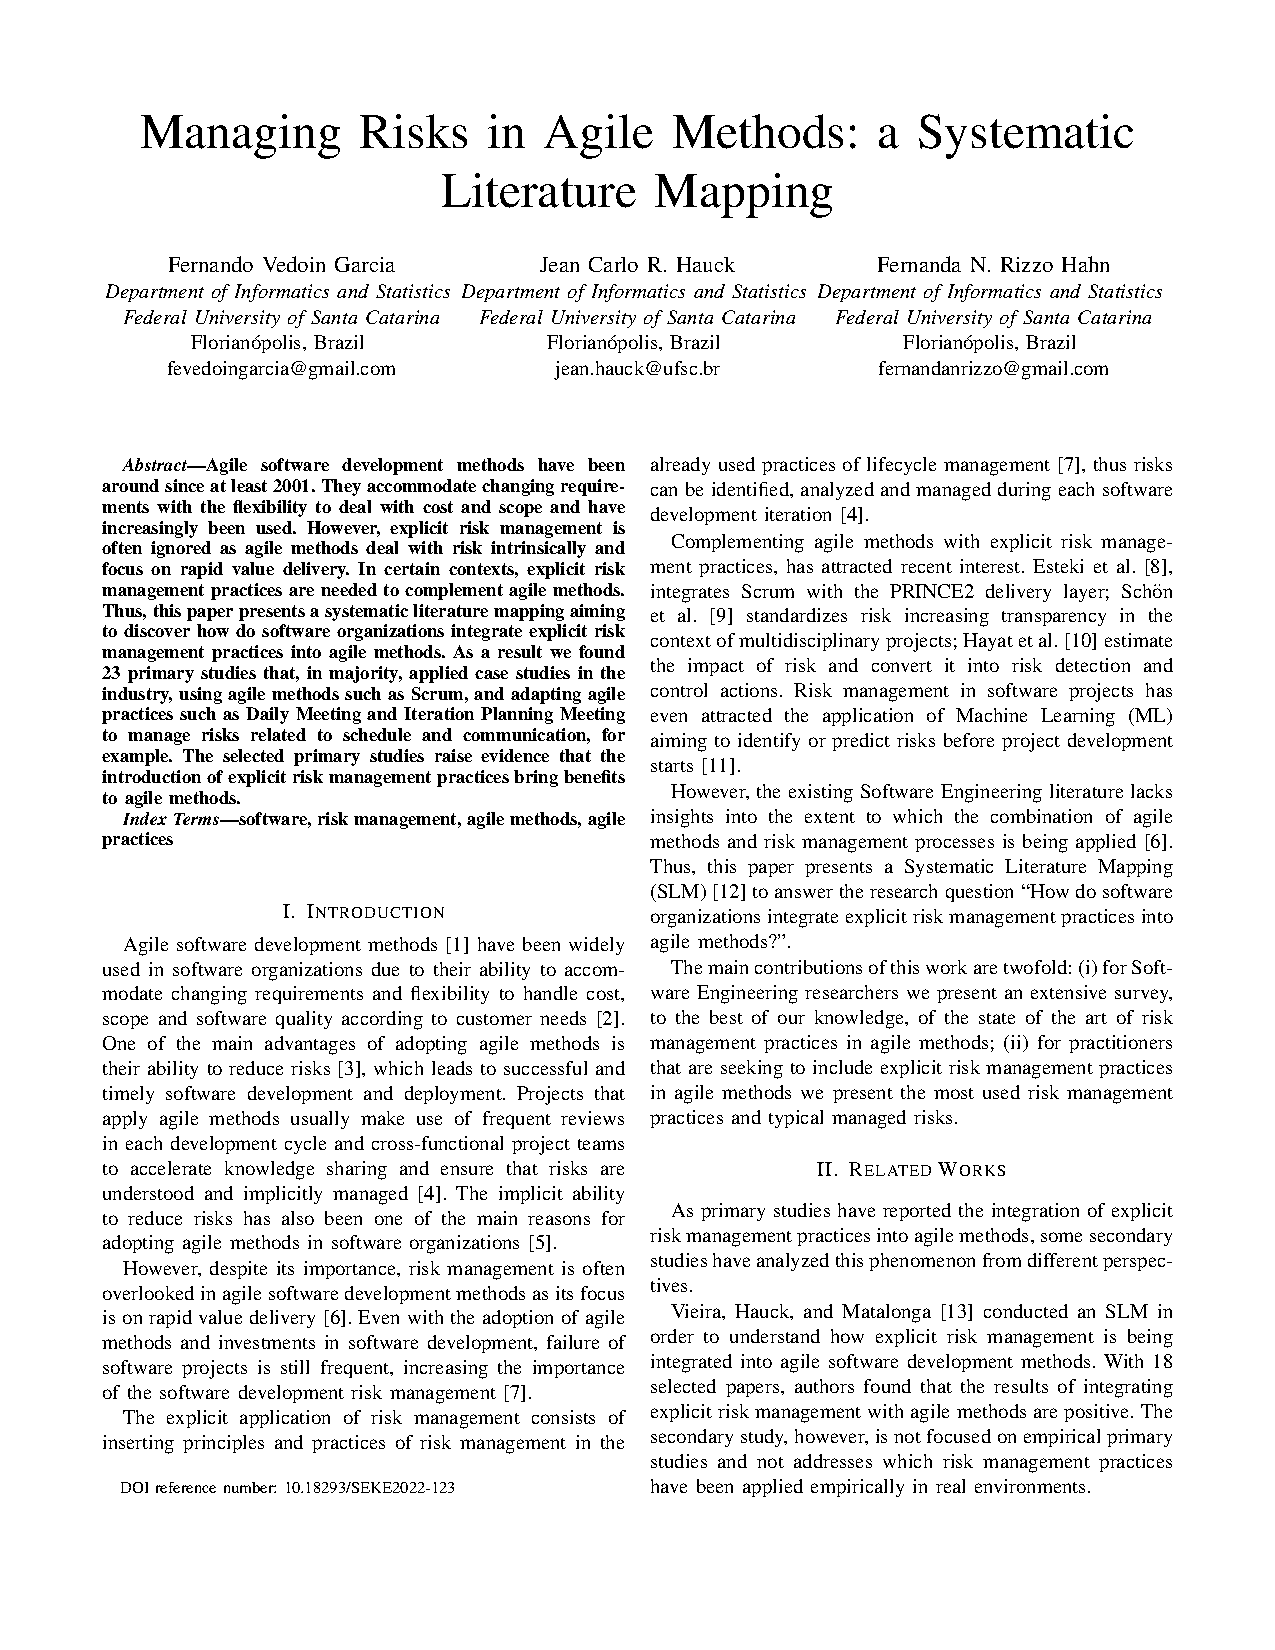
\includepdf[pages=-]{artigo.pdf}

  \end{apendicesenv}
  % ---
  % ----------------------------------------------------------
  % Anexos
  % ----------------------------------------------------------

  % ---
  % Inicia os anexos
  % ---
   \begin{anexosenv}

  % Imprime uma página indicando o início dos anexos
   \partanexos

   \chapter{Declaração de Concordância}
    \label{sec:anexoA}
    \centering
    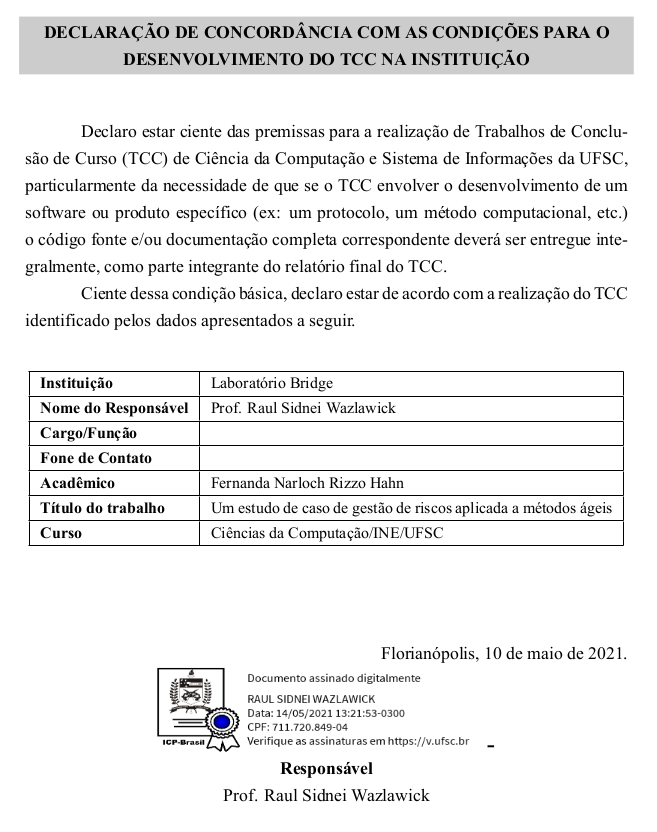
\includegraphics[scale=0.75]{src/tex/declaracao.png}


   \end{anexosenv}

  %---------------------------------------------------------------------
  % INDICE REMISSIVO
  %---------------------------------------------------------------------

  \printindex

  \end{document}
